 %%%%%%%%%%%%%%%%%%%%%%%%%%%%%%%%%%%%%%%%%%%%%%%%%%%%%%%%%%%%
%% This Beamer template was created by Cameron Bracken.
%% Anyone can freely use or modify it for any purpose
%% without attribution.
%%
%% Last Modified: January 9, 2009
%%
\documentclass[xcolor=x11names,compress,t]{beamer}
\usepackage{algorithm,algorithmic, color, tikz}
%% General document %%%%%%%%%%%%%%%%%%%%%%%%%%%%%%%%%
%%\usepackage{tikz}

\usepackage{array}
\usepackage{booktabs}

\usepackage{amssymb}% http://ctan.org/pkg/amssymb
\usepackage{pifont}% http://ctan.org/pkg/pifont
\newcommand{\cmark}{{\color{blue}\selectfont \ding{51}} \vspace{.2 cm}}%
\newcommand{\xmark}{{\color{red}\selectfont \ding{55}} \vspace{.18 cm}}%

\usepackage[makeroom]{cancel}
\usepackage[normalem]{ulem}
\usepackage{verbatim}
\usetikzlibrary{arrows,shapes,arrows.meta,calc,decorations.pathreplacing,positioning}

\newcommand{\even}[0]{\text{Even}}
\newcommand{\odd}[0]{\text{Odd}}
\newcommand{\negg}[0]{\text{Neg}}
\newcommand{\poss}[0]{\text{Pos}}

\newcommand{\match}[3]{
\item {\textbf{#1}\newline Appears #2 times. Example match: \\\{#3\} \newline}
}
\newcommand{\matchone}[2]{
\item {\textbf{#1}\newline Match: \{#2\} \newline}
}

%\usepackage{silence}
\usepackage{graphicx}
\usepackage{epstopdf}
\usepackage{ragged2e}
\usepackage{soul}
%\usepackage[all, cmtip]{xy}
%\usepackage{tikz}
%\usetikzlibrary{decorations.fractals}
%%%%%%%%%%%%%%%%%%%%%%%%%%%%%%%%%%%%%%%%%%%%%%%%%%%%%%

\newcommand{\g}{\mathfrak{g}}
\newcommand{\CC}{\mathbb{C}}
\newcommand{\ot}{\otimes}
\newcommand{\id}{\operatorname{id}}
\newcommand{\bt}{\boxtimes}
\newcommand{\ZZ}{\mathbb{Z}}
\newcommand{\cO}{\mathcal{O}}
\newcommand{\cD}{\mathcal{D}}
\newcommand{\dd}{\mathbf{d}}
\newcommand{\ev}{\operatorname{ev}}

\def\HH{\hbox{${\mathcal H}$\kern-5.2pt${\mathcal H}$}}
\newcommand{\Mat}{\operatorname{Mat}}
\setbeamertemplate{navigation symbols}{}
\setbeamercolor{block title}{bg=blue!40}
\setbeamercolor{block body}{bg=blue!20}

%\usepackage{refcheck}
%\ErrorFilter{xy}{No room for a new}
%\usepackage[all,cmtip,curve, knot,frame]{xy}
\usepackage{amssymb}
\usepackage{amsfonts}
\usepackage{latexsym}
\usetikzlibrary{matrix}
\usepackage{mathabx}
%% Beamer Layout %%%%%%%%%%%%%%%%%%%%%%%%%%%%%%%%%%

\useoutertheme[subsection=false,shadow]{miniframes}
\useinnertheme{default}
\usefonttheme{serif}
\usepackage{palatino}
\setbeamerfont{title like}{shape=\scshape}
\setbeamerfont{frametitle}{shape=\scshape}
\setbeamercolor*{lower separation line head}{bg=DeepSkyBlue4}
\setbeamercolor*{normal text}{fg=black,bg=white}
\setbeamercolor*{alerted text}{fg=red}
\setbeamercolor*{example text}{fg=black}
\setbeamercolor*{structure}{fg=black}
\setbeamercolor*{palette tertiary}{fg=black,bg=black!10}
\setbeamercolor*{palette quaternary}{fg=black,bg=black!10}
\renewcommand{\(}{\begin{columns}}
\renewcommand{\)}{\end{columns}}
\newcommand{\<}[1]{\begin{column}{#1}}
\renewcommand{\>}{\end{column}}
\newcommand{\rot}{\operatorname*{rot}}
\newtheorem{remark}{Remark}
\newtheorem{thm}{Theorem}
\newtheorem{defn}{Definition}
\newtheorem{lem}{Lemma}
\newtheorem{cor}{Corollary}
\newtheorem{conj}{Conjecture}
\newtheorem{problemstatement}{Problem}
\usepackage{hanging}
\setbeamertemplate{footnote}{\hangpara{2em}{1}\makebox[2em][l]{\insertfootnotemark}\scriptsize\insertfootnotetext\par}

\def \av {\text{AV}}
\newcommand{\bb}[1]{\color{blue} #1}
\newcommand{\rr}[1]{\color{red} #1}
\newcommand{\gr}[1]{\color{gray} #1}
\newcommand{\bin}[0]{\text{Bin}}
\newcommand{\ed}[0]{\operatorname{ed}}
\newcommand{\xpivot}[0]{\text{xpivot}}
\newcommand{\ypivot}[0]{\text{ypivot}}
\newcommand{\ypivotopt}[0]{\text{ypivot}_{\text{opt}}}
\def \av {\text{AV}}
\renewcommand{\epsilon}{\varepsilon}
%%%%%%%%%%%%%%%%%%%%%%%%%%%%%%%%%%%%%%%%%%%%%%%%%%
\usepackage[utf8]{inputenc}
\usepackage[T1]{fontenc}
\usepackage{soul}

% ---------- TikZ helpers for Two-World slides (improved) ----------
% Dimensions (scaled down for better fit)
\def\binw{0.9}
\def\binh{0.3}
\def\bingap{0.35}
\def\biny{-1.9}
\def\ballsize{0.52cm}
\def\ballspacing{0.625}

% World positions so that the bin groups are centered in the left/right halves
% of the slide, using Beamer's default \paperwidth = 12.8cm.
% We model the slide width as [-6.4,6.4] in our x-coordinates (1 unit = 1cm),
% so the 25% and 75% positions are at x = -3.2 and x = +3.2.
% Each group has width W = 4*(\binw) + 3*(\bingap) = 4.65, so the starting
% x-positions are center - W/2.
\def\xL{-5.525} % left world: [-5.525, -0.875], centered at -3.2
\def\xR{0.875}  % right world: [0.875, 5.525], centered at +3.2

\newcommand{\DrawBinsAt}[1]{% xstart
  \foreach \i in {0,1,2,3}{
    \pgfmathsetmacro{\x}{#1 + \i*(\binw+\bingap)}
    % Draw bin as open-top container with slight rounded corners
    \draw[line width=1pt, black!80] (\x,\biny) -- (\x,\binh);
    \draw[line width=1pt, black!80] ({\x+\binw},\biny) -- ({\x+\binw},\binh);
    \draw[line width=1pt, black!80] (\x,\biny) -- ({\x+\binw},\biny);
  }
}

\newcommand{\BallInBin}[5]{% xstart, bin(1-4), level(1..), tikz style, text
  \pgfmathsetmacro{\xx}{#1+(#2-1)*(\binw+\bingap)+0.5*\binw}
  \pgfmathsetmacro{\yy}{\biny+0.35+(#3-1)*\ballspacing}
  \node[circle, draw, minimum size=\ballsize, inner sep=0pt, line width=0.8pt, fill=black!15, #4] at (\xx,\yy) {\scriptsize #5};
}

\newcommand{\BinTop}[3]{% xstart, bin(1-4), name
  \pgfmathsetmacro{\tx}{#1+(#2-1)*(\binw+\bingap)+0.5*\binw}
  \coordinate (#3) at (\tx,{\binh-0.1});
}

\newcommand{\TopSeq}{}% Now integrated into TwoWorldFigure

\newcommand{\TwoWorldFigure}[3][0]{% [recourse count] extra tikz for world0 balls, world1 balls
  % Center the entire picture with respect to the full slide width (\paperwidth).
  % Shift left by half of (paperwidth - textwidth) to compensate for the theme's
  % right-shift of the text area.
  \noindent\hspace*{-0.5\dimexpr\paperwidth-\textwidth\relax}%
  \makebox[\paperwidth][c]{%
  \begin{tikzpicture}[x=1cm,y=1cm,scale=0.95]
    % Fix the bounding box to be symmetric around x=0 with total width equal
    % to Beamer's default \paperwidth = 12.8cm, i.e., [-6.4,6.4].
    \path[use as bounding box] (-6.4,-3.0) rectangle (6.4,3.0);
    % Debug guide (commented out):
    % \draw[dashed, very thin, gray!50] (-6.4,-3.0) rectangle (6.4,3.0);
    % separator line
    \draw[dash pattern=on 4pt off 3pt, line width=0.8pt, black!35] (0,-2.8) -- (0,2.8);

    % bins for both worlds
    \DrawBinsAt{\xL}
    \DrawBinsAt{\xR}

    % S_0 and S_1 labels removed for cleaner look - the animation shows insertions step by step
    % \node[font=\small, anchor=north] at ({\xL+1.5*(\binw+\bingap)+0.5*\binw},2.8) {$S_0 = x_1,x_2,x_3,x_4,\ldots$};
    % \node[font=\small, anchor=north] at ({\xR+1.5*(\binw+\bingap)+0.5*\binw},2.8) {$S_1 = x_1,x_2,x_3,x_4,{\color{blue}x},\ldots$};

    % world labels below bins
    \node[font=\normalsize] at ({\xL+1.5*(\binw+\bingap)+0.5*\binw},-2.45) {Computing $A_S$};
    \node[font=\normalsize] at ({\xR+1.5*(\binw+\bingap)+0.5*\binw},-2.45) {Computing $A_{S \cup \{x\}}$};
    
    % Recourse counter in top right
    \node[font=\normalsize, anchor=north east] at (6.2, 2.8) {Recourse $= #1$};

    % bin-top coords for arrows
    \foreach \b in {1,2,3,4}{
      \BinTop{\xL}{\b}{LT\b}
      \BinTop{\xR}{\b}{RT\b}
    }

    % balls (passed in via arguments)
    #2
    #3
  \end{tikzpicture}
  }%
  \vspace{-2mm}
}

% styles for Two-World slides (improved colors)
\tikzset{
  RedBallStyle/.style={draw=black, fill=black!15, text=black!70, line width=0.9pt},
  BlueOutlineStyle/.style={draw=green!50!black, fill=green!20, text=green!50!black, line width=0.9pt},
  BlueFillStyle/.style={fill=blue!70, draw=blue!90!black, text=white, line width=0.9pt}
}

\begin{document}

\begin{frame}[plain]
  \vspace{5mm}
  \begin{center}
    {\LARGE \textbf{History-Independent Load Balancing}}
  \end{center}
  
  \vspace{6mm}
  
  \begin{center}
  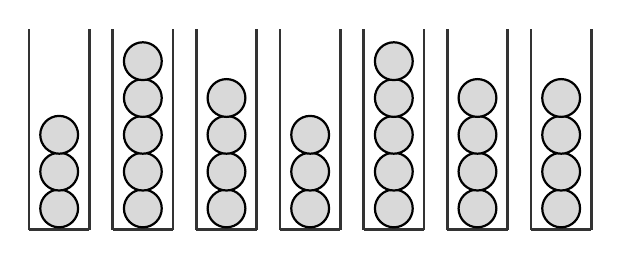
\begin{tikzpicture}[scale=0.85]
    % Exact same dimensions as Two-Choice Load Balancing slide
    \def\bw{0.9}
    \def\bh{3.0}
    \def\by{0}
    \def\bgap{0.35}
    \def\bs{0.48cm}
    \def\bsp{0.55}
    
    % Draw 7 rectangular bins
    \foreach \i in {0,...,6} {
      \pgfmathsetmacro{\xx}{\i*(\bw+\bgap)}
      \draw[line width=1pt, black!80] (\xx,\by) -- (\xx,\bh);
      \draw[line width=1pt, black!80] ({\xx+\bw},\by) -- ({\xx+\bw},\bh);
      \draw[line width=1pt, black!80] (\xx,\by) -- ({\xx+\bw},\by);
    }
    
    % Bin 0: 3 balls
    \foreach \j in {1,2,3} {
      \pgfmathsetmacro{\bx}{0*(\bw+\bgap)+0.5*\bw}
      \pgfmathsetmacro{\byy}{\by+0.32+(\j-1)*\bsp}
      \node[circle, draw, minimum size=\bs, inner sep=0pt, line width=0.8pt, fill=black!15] at (\bx,\byy) {};
    }
    % Bin 1: 5 balls
    \foreach \j in {1,2,3,4,5} {
      \pgfmathsetmacro{\bx}{1*(\bw+\bgap)+0.5*\bw}
      \pgfmathsetmacro{\byy}{\by+0.32+(\j-1)*\bsp}
      \node[circle, draw, minimum size=\bs, inner sep=0pt, line width=0.8pt, fill=black!15] at (\bx,\byy) {};
    }
    % Bin 2: 4 balls
    \foreach \j in {1,2,3,4} {
      \pgfmathsetmacro{\bx}{2*(\bw+\bgap)+0.5*\bw}
      \pgfmathsetmacro{\byy}{\by+0.32+(\j-1)*\bsp}
      \node[circle, draw, minimum size=\bs, inner sep=0pt, line width=0.8pt, fill=black!15] at (\bx,\byy) {};
    }
    % Bin 3: 3 balls
    \foreach \j in {1,2,3} {
      \pgfmathsetmacro{\bx}{3*(\bw+\bgap)+0.5*\bw}
      \pgfmathsetmacro{\byy}{\by+0.32+(\j-1)*\bsp}
      \node[circle, draw, minimum size=\bs, inner sep=0pt, line width=0.8pt, fill=black!15] at (\bx,\byy) {};
    }
    % Bin 4: 5 balls
    \foreach \j in {1,2,3,4,5} {
      \pgfmathsetmacro{\bx}{4*(\bw+\bgap)+0.5*\bw}
      \pgfmathsetmacro{\byy}{\by+0.32+(\j-1)*\bsp}
      \node[circle, draw, minimum size=\bs, inner sep=0pt, line width=0.8pt, fill=black!15] at (\bx,\byy) {};
    }
    % Bin 5: 4 balls
    \foreach \j in {1,2,3,4} {
      \pgfmathsetmacro{\bx}{5*(\bw+\bgap)+0.5*\bw}
      \pgfmathsetmacro{\byy}{\by+0.32+(\j-1)*\bsp}
      \node[circle, draw, minimum size=\bs, inner sep=0pt, line width=0.8pt, fill=black!15] at (\bx,\byy) {};
    }
    % Bin 6: 4 balls
    \foreach \j in {1,2,3,4} {
      \pgfmathsetmacro{\bx}{6*(\bw+\bgap)+0.5*\bw}
      \pgfmathsetmacro{\byy}{\by+0.32+(\j-1)*\bsp}
      \node[circle, draw, minimum size=\bs, inner sep=0pt, line width=0.8pt, fill=black!15] at (\bx,\byy) {};
    }
  \end{tikzpicture}
  \end{center}
  
  \vspace{6mm}
  
  \begin{center}
  \begin{tabular}{@{}c@{\hspace{8mm}}c@{\hspace{8mm}}c@{\hspace{8mm}}c@{}}
    {\footnotesize Michael A.\ Bender} &
    {\footnotesize William Kuszmaul} &
    {\footnotesize Elaine Shi} &
    {\footnotesize \textbf{Rose Silver}} \\[1mm]
    {\scriptsize Stony Brook University} &
    {\scriptsize CMU} &
    {\scriptsize CMU} &
    {\scriptsize CMU}
  \end{tabular}
  \end{center}
\end{frame}


\begin{frame}{NYT Censoring Catastrophe}
  \pause
  \vspace{-0.2cm}
  \begin{center}
  \includegraphics[width=0.65\textwidth]{nyt.png}
  \end{center}
  \vspace{-0.3cm}
  \begin{itemize}\setlength{\itemsep}{2pt}

    \item \textbf{2000:} NYT publishes internal CIA report \pause
    % \item Final state redacted successfully
    \item However, during rendering, the hidden text could be captured
  \end{itemize}
  \pause
  \vspace{0.4cm}
  \begin{center}
    \large\textbf{History can be just as important as content!}
  \end{center}
\end{frame}


% --- Data Structure Concept Slide (with animation) ---
\begin{frame}{History-Independent Data Structures}

\hspace*{-1cm}
\begin{tikzpicture}[scale=0.65]
  
  \def\h{2.5}
  \def\hh{0}
  \def\hhh{-2.5}
  \def\sp{3.8} % horizontal spacing between circles
  
  % Extend height for consistent layout
  \path (-2.5, -3.2) -- (-2.5, 3.5);
  
  % === History 1: appears on frame 2+ ===
  \only<2->{
    % Label
    \node[font=\small, gray] at (-2.5, \h) {History 1:};
    
    % First three circles (always grey)
    \node[draw, circle, minimum size=1.1cm, fill=black!5, line width=1pt] (h1s0) at (0, \h) {\small $\emptyset$};
    \node[draw, circle, minimum size=1.1cm, fill=black!5, line width=1pt] (h1s1) at (\sp, \h) {\small $\{x\}$};
    \node[draw, circle, minimum size=1.1cm, fill=black!5, line width=1pt] (h1s2) at (2*\sp, \h) {\small $\{x,y\}$};
    
    % Arrows
    \draw[-{Stealth[length=2mm, width=1.5mm]}, black!60, line width=1pt] 
      (h1s0.east) to[out=30, in=150] (h1s1.west);
    \node[black!60, font=\normalsize] at (0.5*\sp, \h+0.7) {$+x$};
    \draw[-{Stealth[length=2mm, width=1.5mm]}, black!60, line width=1pt] 
      (h1s1.east) to[out=30, in=150] (h1s2.west);
    \node[black!60, font=\normalsize] at (1.5*\sp, \h+0.7) {$+y$};
  }
  
  % Last circle: grey on frame 2, blue on frames 3+
  \only<2>{\node[draw, circle, minimum size=1.1cm, fill=black!5, line width=1pt] (h1s3grey) at (3*\sp, \h) {\small $\{y\}$};}
  \only<3->{\node[draw, circle, minimum size=1.1cm, fill=blue!15, draw=blue!70!black, line width=1pt] (h1s3grey) at (3*\sp, \h) {\small $\{y\}$};}
  
  % Delete arrow (appears with History 1)
  \only<2->{
    \draw[-{Stealth[length=2mm, width=1.5mm]}, black!60, line width=1pt] 
      (h1s2.east) to[out=30, in=150] (h1s3grey.west);
    \node[black!60, font=\normalsize] at (2.5*\sp, \h+0.7) {$-x$};
  }
  
  % === Adversary on the right side (appears on frame 3+) ===
  \only<3->{
    \node[font=\small, blue, overlay] (adv) at (3*\sp + 2.5, \h - 2.5) {\textbf{Adversary}};
    \draw[overlay, -{Stealth[length=2.5mm, width=2mm]}, blue, line width=1.2pt] 
      (adv.north) -- (h1s3grey.south east);
  }
  
  % === History 2: Insert(y), Insert(x), Delete(x) - appears on frame 5+ ===
  \only<5->{
    \node[font=\small, gray] at (-2.5, \hh) {History 2:};
    \node[draw, circle, minimum size=1.1cm, fill=black!5, line width=1pt] (h2s0) at (0, \hh) {\small $\emptyset$};
    \node[draw, circle, minimum size=1.1cm, fill=black!5, line width=1pt] (h2s1) at (\sp, \hh) {\small $\{y\}$};
    \node[draw, circle, minimum size=1.1cm, fill=black!5, line width=1pt] (h2s2) at (2*\sp, \hh) {\small $\{x,y\}$};
    \node[draw, circle, minimum size=1.1cm, fill=blue!15, draw=blue!70!black, line width=1pt] (h2s3) at (3*\sp, \hh) {\small $\{y\}$};
    
    \draw[-{Stealth[length=2mm, width=1.5mm]}, red!70!black, line width=1pt] 
      (h2s0.east) to[out=30, in=150] (h2s1.west);
    \node[red!70!black, font=\normalsize\bfseries] at (0.5*\sp, \hh+0.7) {$+y$};
    \draw[-{Stealth[length=2mm, width=1.5mm]}, red!70!black, line width=1pt] 
      (h2s1.east) to[out=30, in=150] (h2s2.west);
    \node[red!70!black, font=\normalsize\bfseries] at (1.5*\sp, \hh+0.7) {$+x$};
    \draw[-{Stealth[length=2mm, width=1.5mm]}, black!60, line width=1pt] 
      (h2s2.east) to[out=30, in=150] (h2s3.west);
    \node[black!60, font=\normalsize] at (2.5*\sp, \hh+0.7) {$-x$};
  }
  
  % === History 3: ... -> {y} -> Insert(z) -> {y,z} -> Delete(z) -> {y} - appears on frame 6+ ===
  \only<6->{
    \node[font=\small, gray] at (-2.5, \hhh) {History 3:};
    \node[draw, circle, minimum size=1.1cm, fill=black!5, line width=1pt] (h3s0) at (0, \hhh) {\small $\emptyset$};
    \node[draw, circle, minimum size=1.1cm, fill=black!5, line width=1pt] (h3s1) at (\sp, \hhh) {\small $\{y\}$};
    \node[draw, circle, minimum size=1.1cm, fill=black!5, line width=1pt] (h3s2) at (2*\sp, \hhh) {\small $\{y,z\}$};
    \node[draw, circle, minimum size=1.1cm, fill=blue!15, draw=blue!70!black, line width=1pt] (h3s3) at (3*\sp, \hhh) {\small $\{y\}$};
    
    \draw[-{Stealth[length=2mm, width=1.5mm]}, gray, line width=1pt, dashed] 
      (h3s0.east) -- (h3s1.west);
    \node[gray, font=\scriptsize] at (0.5*\sp, \hhh+0.35) {$\cdots$};
    \draw[-{Stealth[length=2mm, width=1.5mm]}, black!60, line width=1pt] 
      (h3s1.east) to[out=30, in=150] (h3s2.west);
    \node[black!60, font=\normalsize] at (1.5*\sp, \hhh+0.7) {$+z$};
    \draw[-{Stealth[length=2mm, width=1.5mm]}, black!60, line width=1pt] 
      (h3s2.east) to[out=30, in=150] (h3s3.west);
    \node[black!60, font=\normalsize] at (2.5*\sp, \hhh+0.7) {$-z$};
  }
  
\end{tikzpicture}

\vfill

\only<4->{
\begin{minipage}{0.95\textwidth}
\textbf{History Independence} {\scriptsize \color{blue}(Micciancio '97, Naor \& Teague '01)}

\vspace{0.1cm}
\begin{itemize}
\item The state reveals only the current elements—\textbf{not the history of operations.}
\end{itemize}
\end{minipage}
}

\end{frame}


% \begin{frame}{History Independent Data Structures}

% \vfill

% \begin{center}
% \begin{minipage}{0.85\textwidth}
% \textbf{History Independence} {\small \color{blue}(Micciancio '97, Naor \& Teague '01)}

% \vspace{0.4cm}
% \hspace{0.5cm}\begin{minipage}{0.9\textwidth}
% \textit{``If an adversary were to see the state of the data structure,
% they would learn only the current set of elements, and nothing else about the history of past operations.''}
% \end{minipage}
% \end{minipage}
% \end{center}

% \vfill

% \end{frame}



% \begin{frame}{History vs Content}

% \(
% \<{0.35\textwidth}
%   \begin{center}
%   \includegraphics[height = 8 cm]{./contacts.jpg}
%   \end{center}
% \>
% \<{0.65\textwidth}
% \begin{itemize}
% \item If someone hacks my phone, they can learn my contacts list. \pause

% \vspace{0.5 cm}

% \item But can they learn who my contacts were in the past? \pause

% \vspace{0.5 cm}
  
% \item What about the order in which contacts were added? \pause

% \vspace{0.5 cm}

% \item A history independent data structure protects this kind of information.
% \end{itemize}
% \>
% \)
% \end{frame}



\begin{frame}{History Independent Data Structures}

% \vspace{0.8cm}

% \textbf{History Independence} {\small \color{blue}(Micciancio '97, Naor \& Teague '01)}

% \vspace{0.3cm}
% \hspace{0.5cm}\begin{minipage}{0.9\textwidth}
% \textit{``If an adversary were to see the state of the data structure,
% they would learn only the current set of elements, and nothing else about the history of past operations.''}
% \end{minipage}

% \pause
% \vspace{0.6cm}

\textbf{A History of Applications}

\vspace{0.3cm}
\hspace{0.5cm}\begin{minipage}{0.9\textwidth}
Hash tables, trees, memory allocation, PMAs, graph algorithms, cache-oblivious data structures, and more.\\[0.2cm]
{\tiny \color{blue} Micciancio '97, Naor \& Teague '01, Buchbinder \& Petrank '03, Molnar et al.~'06, Blelloch \& Golovin '07, Moran et al.~'07, Naor et al.~'08, Golovin '08--'10, Bajaj \& Sion '13, Roche et al.~'15, Bender et al.~'16}
\end{minipage}

\pause
\vspace{0.6cm}

\textbf{Yet some basic questions remain open.}

\vspace{0.5cm}
\pause

\textbf{This work:} History-Independent Load Balancing

\end{frame}

% --- Old cup-style slide (commented out) ---
% \begin{frame}{Two-Choice Load Balancing}
% 
% \begin{center}
% \begin{tikzpicture}[scale=0.8]
%   % Define bin dimensions
%   \def\binwidth{0.6}
%   \def\binheight{2.5}
%   \def\ballradius{0.2}
%   \def\binspacing{1.0}
%   
%   % Draw 7 bins as cups (bottom line + two small side lines)
%   \def\sideheight{0.15}
%   \foreach \i in {0,...,6} {
%     \draw[thick] (\i*\binspacing, \sideheight) -- (\i*\binspacing, 0) -- (\i*\binspacing + \binwidth, 0) -- (\i*\binspacing + \binwidth, \sideheight);
%   }
%   
%   % Add balls to bins (varying amounts, average ~4)
%   % Bin 0: 3 balls
%   \foreach \j in {1,2,3} {
%     \fill[black] (0*\binspacing + \binwidth/2, \j*0.45 - 0.1) circle (\ballradius);
%   }
%   % Bin 1: 5 balls
%   \foreach \j in {1,2,3,4,5} {
%     \fill[black] (1*\binspacing + \binwidth/2, \j*0.45 - 0.1) circle (\ballradius);
%   }
%   % Bin 2: 4 balls
%   \foreach \j in {1,2,3,4} {
%     \fill[black] (2*\binspacing + \binwidth/2, \j*0.45 - 0.1) circle (\ballradius);
%   }
%   % Bin 3: 3 balls
%   \foreach \j in {1,2,3} {
%     \fill[black] (3*\binspacing + \binwidth/2, \j*0.45 - 0.1) circle (\ballradius);
%   }
%   % Bin 4: 5 balls
%   \foreach \j in {1,2,3,4,5} {
%     \fill[black] (4*\binspacing + \binwidth/2, \j*0.45 - 0.1) circle (\ballradius);
%   }
%   % Bin 5: 4 balls
%   \foreach \j in {1,2,3,4} {
%     \fill[black] (5*\binspacing + \binwidth/2, \j*0.45 - 0.1) circle (\ballradius);
%   }
%   % Bin 6: 4 balls
%   \foreach \j in {1,2,3,4} {
%     \fill[black] (6*\binspacing + \binwidth/2, \j*0.45 - 0.1) circle (\ballradius);
%   }
%   
%   % Ball x being inserted (same size as other balls, centered)
%   \fill[black] (3*\binspacing + \binwidth/2, 3.5) circle (\ballradius);
%   \node[above] at (3*\binspacing + \binwidth/2, 3.5 + \ballradius) {$x$};
%   
%   % Arrows to h_1(x) and h_2(x) - pointing to bin 1 and bin 3 (second and fourth)
%   \draw[->, thick] (3*\binspacing + \binwidth/2 - 0.1, 3.5 - \ballradius) to[out=-150, in=90] (1*\binspacing + \binwidth/2, \binheight + 0.1);
%   \node[left] at (1.5, 3.1) {$h_1(x)$};
%   \draw[->, thick] (3*\binspacing + \binwidth/2 + 0.1, 3.5 - \ballradius) to[out=-50, in=90] (3*\binspacing + \binwidth/2, 3*0.45 + \ballradius);
%   \node[right] at (3.6, 3.1) {$h_2(x)$};
%   
%   % Label: n bins
%   \draw[<->] (0, -0.4) -- (6*\binspacing + \binwidth, -0.4);
%   \node[below, blue] at (3*\binspacing + \binwidth/2, -0.4) {$n$ bins};
%   
% \end{tikzpicture}
% \end{center}
% 
% 
%   \begin{itemize}
%   \item Balls are {\color{green!50!black}inserted}/{\color{red!70!black}deleted}, with up to {\color{blue}$m$} present at a time.
%   \item Each ball has two random bins where it can go. 
%   \item We must maintain a valid assignment of balls to bins.
%   \end{itemize}
% 
% \end{frame}

% --- New slide with Two-World style bins/balls ---
\begin{frame}{Two-Choice Load Balancing}

\vspace{0.2cm}
\begin{center}
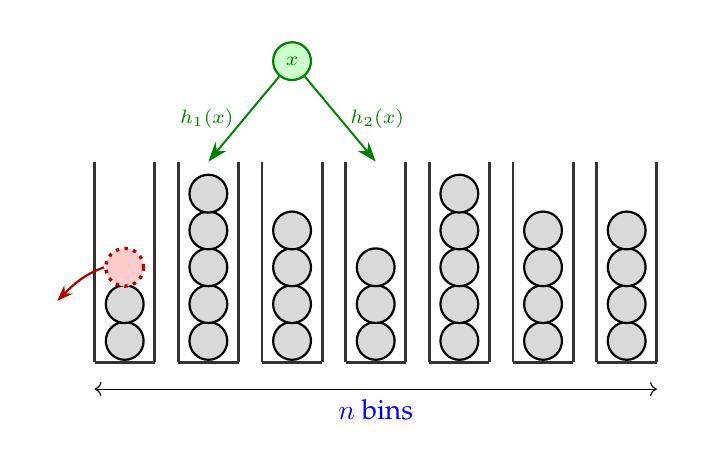
\begin{tikzpicture}[scale=0.85]
  % Dimensions matching Two-World style
  \def\bw{0.9}       % bin width
  \def\bh{3.0}       % bin height (top y) - taller to contain all balls
  \def\by{0}         % bin bottom y
  \def\bgap{0.35}    % gap between bins
  \def\bs{0.48cm}    % ball size
  \def\bsp{0.55}     % ball spacing
  
  % Fixed bounding box to prevent shifting when elements appear
  \path[use as bounding box] (-1, -1) rectangle (9, 5);
  
  % Draw 7 rectangular bins
  \foreach \i in {0,...,6} {
    \pgfmathsetmacro{\xx}{\i*(\bw+\bgap)}
    \draw[line width=1pt, black!80] (\xx,\by) -- (\xx,\bh);
    \draw[line width=1pt, black!80] ({\xx+\bw},\by) -- ({\xx+\bw},\bh);
    \draw[line width=1pt, black!80] (\xx,\by) -- ({\xx+\bw},\by);
  }
  
  % Place balls in bins using foreach
  % Bin 0: 2 balls + 1 being deleted (top)
  \foreach \j in {1,2} {
    \pgfmathsetmacro{\bx}{0*(\bw+\bgap)+0.5*\bw}
    \pgfmathsetmacro{\byy}{\by+0.32+(\j-1)*\bsp}
    \node[circle, draw, minimum size=\bs, inner sep=0pt, line width=0.8pt, fill=black!15] at (\bx,\byy) {};
  }
  % Deleted ball (dotted red) - appears with first bullet point
  \only<2->{
    \pgfmathsetmacro{\delx}{0*(\bw+\bgap)+0.5*\bw}
    \pgfmathsetmacro{\dely}{\by+0.32+(3-1)*\bsp}
    \node[circle, draw, dotted, minimum size=\bs, inner sep=0pt, line width=1.2pt, draw=red!70!black, fill=red!20] (delball) at (\delx,\dely) {};
    % Curved arrow showing ball being thrown out (overlay so it doesn't shift the picture)
    \draw[overlay, -{Stealth[length=2mm, width=1.5mm]}, red!70!black, line width=0.8pt] 
      (delball.west) to[out=200, in=45] ++(-0.7,-0.5);
  }
  % Bin 1: 5 balls
  \foreach \j in {1,2,3,4,5} {
    \pgfmathsetmacro{\bx}{1*(\bw+\bgap)+0.5*\bw}
    \pgfmathsetmacro{\byy}{\by+0.32+(\j-1)*\bsp}
    \node[circle, draw, minimum size=\bs, inner sep=0pt, line width=0.8pt, fill=black!15] at (\bx,\byy) {};
  }
  % Bin 2: 4 balls
  \foreach \j in {1,2,3,4} {
    \pgfmathsetmacro{\bx}{2*(\bw+\bgap)+0.5*\bw}
    \pgfmathsetmacro{\byy}{\by+0.32+(\j-1)*\bsp}
    \node[circle, draw, minimum size=\bs, inner sep=0pt, line width=0.8pt, fill=black!15] at (\bx,\byy) {};
  }
  % Bin 3: 3 balls
  \foreach \j in {1,2,3} {
    \pgfmathsetmacro{\bx}{3*(\bw+\bgap)+0.5*\bw}
    \pgfmathsetmacro{\byy}{\by+0.32+(\j-1)*\bsp}
    \node[circle, draw, minimum size=\bs, inner sep=0pt, line width=0.8pt, fill=black!15] at (\bx,\byy) {};
  }
  % Bin 4: 5 balls
  \foreach \j in {1,2,3,4,5} {
    \pgfmathsetmacro{\bx}{4*(\bw+\bgap)+0.5*\bw}
    \pgfmathsetmacro{\byy}{\by+0.32+(\j-1)*\bsp}
    \node[circle, draw, minimum size=\bs, inner sep=0pt, line width=0.8pt, fill=black!15] at (\bx,\byy) {};
  }
  % Bin 5: 4 balls
  \foreach \j in {1,2,3,4} {
    \pgfmathsetmacro{\bx}{5*(\bw+\bgap)+0.5*\bw}
    \pgfmathsetmacro{\byy}{\by+0.32+(\j-1)*\bsp}
    \node[circle, draw, minimum size=\bs, inner sep=0pt, line width=0.8pt, fill=black!15] at (\bx,\byy) {};
  }
  % Bin 6: 4 balls
  \foreach \j in {1,2,3,4} {
    \pgfmathsetmacro{\bx}{6*(\bw+\bgap)+0.5*\bw}
    \pgfmathsetmacro{\byy}{\by+0.32+(\j-1)*\bsp}
    \node[circle, draw, minimum size=\bs, inner sep=0pt, line width=0.8pt, fill=black!15] at (\bx,\byy) {};
  }
  
  % Ball x being inserted (dark forest green, centered between its two choices) - appears with first bullet point
  \only<2->{
    \pgfmathsetmacro{\binoneX}{1*(\bw+\bgap)+0.5*\bw}
    \pgfmathsetmacro{\binthreeX}{3*(\bw+\bgap)+0.5*\bw}
    \pgfmathsetmacro{\xball}{(\binoneX+\binthreeX)/2}
    \node[circle, draw, minimum size=\bs, inner sep=0pt, line width=0.8pt, draw=green!50!black, fill=green!20, text=green!50!black] (xball) at (\xball,4.5) {\scriptsize $x$};
    
    % Straight arrows to two bins (bin 1 and bin 3) with labels
    \draw[-{Stealth[length=2.5mm, width=1.8mm]}, green!50!black, line width=0.7pt] (xball) -- (\binoneX,\bh) node[midway, left, green!50!black] {\scriptsize $h_1(x)$};
    \draw[-{Stealth[length=2.5mm, width=1.8mm]}, green!50!black, line width=0.7pt] (xball) -- (\binthreeX,\bh) node[midway, right, green!50!black] {\scriptsize $h_2(x)$};
  }
  
  % Label: n bins
  \pgfmathsetmacro{\totalw}{6*(\bw+\bgap)+\bw}
  \draw[<->] (0, -0.4) -- (\totalw, -0.4);
  \node[below, blue] at ({0.5*\totalw}, -0.4) {$n$ bins};
  
\end{tikzpicture}
\end{center}

  \begin{itemize}
  \item<2-> Balls are {\color{green!50!black}inserted}/{\color{red!70!black}deleted}, with up to {\color{blue}$m$} present at a time.
  \item<3-> Each ball has two random bins where it can go. 
  \item<4-> We must maintain a valid assignment of balls to bins.
  \end{itemize}

\end{frame}

% % --- OPTION A: Red dotted ball (no label) ---
% \begin{frame}{Two-Choice Load Balancing}

% \vspace{0.2cm}
% \begin{center}
% \begin{tikzpicture}[scale=0.85]
%   \def\bw{0.9}
%   \def\bh{3.0}
%   \def\by{0}
%   \def\bgap{0.35}
%   \def\bs{0.48cm}
%   \def\bsp{0.55}
  
%   % Draw 7 rectangular bins
%   \foreach \i in {0,...,6} {
%     \pgfmathsetmacro{\xx}{\i*(\bw+\bgap)}
%     \draw[line width=1pt, black!80] (\xx,\by) -- (\xx,\bh);
%     \draw[line width=1pt, black!80] ({\xx+\bw},\by) -- ({\xx+\bw},\bh);
%     \draw[line width=1pt, black!80] (\xx,\by) -- ({\xx+\bw},\by);
%   }
  
%   % Bin 0: 2 balls + 1 being deleted (top)
%   \foreach \j in {1,2} {
%     \pgfmathsetmacro{\bx}{0*(\bw+\bgap)+0.5*\bw}
%     \pgfmathsetmacro{\byy}{\by+0.32+(\j-1)*\bsp}
%     \node[circle, draw, minimum size=\bs, inner sep=0pt, line width=0.8pt, fill=black!15] at (\bx,\byy) {};
%   }
%   % Deleted ball (dotted red, no label)
%   \pgfmathsetmacro{\delx}{0*(\bw+\bgap)+0.5*\bw}
%   \pgfmathsetmacro{\dely}{\by+0.32+(3-1)*\bsp}
%   \node[circle, draw, dotted, minimum size=\bs, inner sep=0pt, line width=1.2pt, draw=red!70!black, fill=red!20] (delball) at (\delx,\dely) {};
%   % Curved arrow showing ball being thrown out (overlay so it doesn't shift the picture)
%   \draw[overlay, -{Stealth[length=2mm, width=1.5mm]}, red!70!black, line width=0.8pt] 
%     (delball.west) to[out=200, in=45] ++(-0.7,-0.5);
  
%   % Remaining bins
%   \foreach \j in {1,2,3,4,5} {
%     \pgfmathsetmacro{\bx}{1*(\bw+\bgap)+0.5*\bw}
%     \pgfmathsetmacro{\byy}{\by+0.32+(\j-1)*\bsp}
%     \node[circle, draw, minimum size=\bs, inner sep=0pt, line width=0.8pt, fill=black!15] at (\bx,\byy) {};
%   }
%   \foreach \j in {1,2,3,4} {
%     \pgfmathsetmacro{\bx}{2*(\bw+\bgap)+0.5*\bw}
%     \pgfmathsetmacro{\byy}{\by+0.32+(\j-1)*\bsp}
%     \node[circle, draw, minimum size=\bs, inner sep=0pt, line width=0.8pt, fill=black!15] at (\bx,\byy) {};
%   }
%   \foreach \j in {1,2,3} {
%     \pgfmathsetmacro{\bx}{3*(\bw+\bgap)+0.5*\bw}
%     \pgfmathsetmacro{\byy}{\by+0.32+(\j-1)*\bsp}
%     \node[circle, draw, minimum size=\bs, inner sep=0pt, line width=0.8pt, fill=black!15] at (\bx,\byy) {};
%   }
%   \foreach \j in {1,2,3,4,5} {
%     \pgfmathsetmacro{\bx}{4*(\bw+\bgap)+0.5*\bw}
%     \pgfmathsetmacro{\byy}{\by+0.32+(\j-1)*\bsp}
%     \node[circle, draw, minimum size=\bs, inner sep=0pt, line width=0.8pt, fill=black!15] at (\bx,\byy) {};
%   }
%   \foreach \j in {1,2,3,4} {
%     \pgfmathsetmacro{\bx}{5*(\bw+\bgap)+0.5*\bw}
%     \pgfmathsetmacro{\byy}{\by+0.32+(\j-1)*\bsp}
%     \node[circle, draw, minimum size=\bs, inner sep=0pt, line width=0.8pt, fill=black!15] at (\bx,\byy) {};
%   }
%   \foreach \j in {1,2,3,4} {
%     \pgfmathsetmacro{\bx}{6*(\bw+\bgap)+0.5*\bw}
%     \pgfmathsetmacro{\byy}{\by+0.32+(\j-1)*\bsp}
%     \node[circle, draw, minimum size=\bs, inner sep=0pt, line width=0.8pt, fill=black!15] at (\bx,\byy) {};
%   }
  
%   % Ball x being inserted (dark forest green)
%   \pgfmathsetmacro{\binoneX}{1*(\bw+\bgap)+0.5*\bw}
%   \pgfmathsetmacro{\binthreeX}{3*(\bw+\bgap)+0.5*\bw}
%   \pgfmathsetmacro{\xball}{(\binoneX+\binthreeX)/2}
%   \node[circle, draw, minimum size=\bs, inner sep=0pt, line width=0.8pt, draw=green!50!black, fill=green!20, text=green!50!black] (xball) at (\xball,4.5) {\scriptsize $x$};
%   \draw[-{Stealth[length=2.5mm, width=1.8mm]}, green!50!black, line width=0.7pt] (xball) -- (\binoneX,\bh) node[midway, left, green!50!black] {\scriptsize $h_1(x)$};
%   \draw[-{Stealth[length=2.5mm, width=1.8mm]}, green!50!black, line width=0.7pt] (xball) -- (\binthreeX,\bh) node[midway, right, green!50!black] {\scriptsize $h_2(x)$};
  
%   \pgfmathsetmacro{\totalw}{6*(\bw+\bgap)+\bw}
%   \draw[<->] (0, -0.4) -- (\totalw, -0.4);
%   \node[below, blue] at ({0.5*\totalw}, -0.4) {$n$ bins};
% \end{tikzpicture}
% \end{center}

%   \begin{itemize}
%   \item Balls are {\color{green!50!black}inserted}/{\color{red!70!black}deleted}, with up to {\color{blue}$m$} present at a time.
%   \item Each ball has two random bins where it can go. 
%   \item We must maintain a valid assignment of balls to bins.
%   \end{itemize}

% \end{frame}

\begin{frame}{Two Goals}

\begin{center}
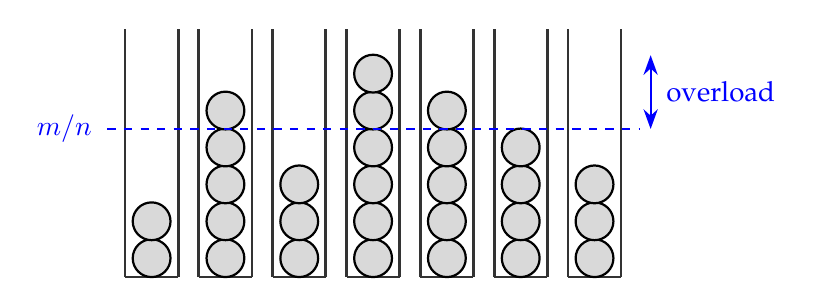
\begin{tikzpicture}[scale=0.75]
  % Dimensions matching Two-World style
  \def\bw{0.9}       % bin width
  \def\bh{4.2}       % bin height (shorter)
  \def\by{0}         % bin bottom y
  \def\bgap{0.35}    % gap between bins
  \def\bs{0.48cm}    % ball size
  \def\bsp{0.625}    % ball spacing (increased to prevent overlap)
  \def\bstart{0.32}  % first ball center offset from bottom
  
  % Draw 7 rectangular bins
  \foreach \i in {0,...,6} {
    \pgfmathsetmacro{\xx}{\i*(\bw+\bgap)}
    \draw[line width=1pt, black!80] (\xx,\by) -- (\xx,\bh);
    \draw[line width=1pt, black!80] ({\xx+\bw},\by) -- ({\xx+\bw},\bh);
    \draw[line width=1pt, black!80] (\xx,\by) -- ({\xx+\bw},\by);
  }
  
  % Add balls to bins (reduced counts to fit shorter bins, m/n ~ 4)
  % Bin 0: 2 balls
  \foreach \j in {1,2} {
    \pgfmathsetmacro{\bx}{0*(\bw+\bgap)+0.5*\bw}
    \pgfmathsetmacro{\byy}{\by+\bstart+(\j-1)*\bsp}
    \node[circle, draw, minimum size=\bs, inner sep=0pt, line width=0.8pt, fill=black!15] at (\bx,\byy) {};
  }
  % Bin 1: 5 balls (above average)
  \foreach \j in {1,2,3,4,5} {
    \pgfmathsetmacro{\bx}{1*(\bw+\bgap)+0.5*\bw}
    \pgfmathsetmacro{\byy}{\by+\bstart+(\j-1)*\bsp}
    \node[circle, draw, minimum size=\bs, inner sep=0pt, line width=0.8pt, fill=black!15] at (\bx,\byy) {};
  }
  % Bin 2: 3 balls
  \foreach \j in {1,2,3} {
    \pgfmathsetmacro{\bx}{2*(\bw+\bgap)+0.5*\bw}
    \pgfmathsetmacro{\byy}{\by+\bstart+(\j-1)*\bsp}
    \node[circle, draw, minimum size=\bs, inner sep=0pt, line width=0.8pt, fill=black!15] at (\bx,\byy) {};
  }
  % Bin 3: 6 balls (the most overloaded bin!)
  \foreach \j in {1,2,3,4,5,6} {
    \pgfmathsetmacro{\bx}{3*(\bw+\bgap)+0.5*\bw}
    \pgfmathsetmacro{\byy}{\by+\bstart+(\j-1)*\bsp}
    \node[circle, draw, minimum size=\bs, inner sep=0pt, line width=0.8pt, fill=black!15] at (\bx,\byy) {};
  }
  % Bin 4: 5 balls (above average)
  \foreach \j in {1,2,3,4,5} {
    \pgfmathsetmacro{\bx}{4*(\bw+\bgap)+0.5*\bw}
    \pgfmathsetmacro{\byy}{\by+\bstart+(\j-1)*\bsp}
    \node[circle, draw, minimum size=\bs, inner sep=0pt, line width=0.8pt, fill=black!15] at (\bx,\byy) {};
  }
  % Bin 5: 4 balls
  \foreach \j in {1,2,3,4} {
    \pgfmathsetmacro{\bx}{5*(\bw+\bgap)+0.5*\bw}
    \pgfmathsetmacro{\byy}{\by+\bstart+(\j-1)*\bsp}
    \node[circle, draw, minimum size=\bs, inner sep=0pt, line width=0.8pt, fill=black!15] at (\bx,\byy) {};
  }
  % Bin 6: 3 balls
  \foreach \j in {1,2,3} {
    \pgfmathsetmacro{\bx}{6*(\bw+\bgap)+0.5*\bw}
    \pgfmathsetmacro{\byy}{\by+\bstart+(\j-1)*\bsp}
    \node[circle, draw, minimum size=\bs, inner sep=0pt, line width=0.8pt, fill=black!15] at (\bx,\byy) {};
  }
  
  % m/n line: average is 4 balls, so line goes between ball 4 and ball 5
  % Position: halfway between 4th ball center and 5th ball center
  \pgfmathsetmacro{\avgheight}{\by+\bstart+(4-1)*\bsp + 0.5*\bsp}
  \pgfmathsetmacro{\totalw}{6*(\bw+\bgap)+\bw}
  \draw[dashed, thick, blue] (-0.3, \avgheight) -- ({\totalw + 0.3}, \avgheight);
  \node[left, blue] at (-0.4, \avgheight) {$m/n$};
  
  % Overload bracket on the right side (exactly 2 ball heights)
  \pgfmathsetmacro{\overloadtop}{\avgheight + 2*\bsp}
  \draw[{Stealth[length=2.5mm, width=1.8mm]}-{Stealth[length=2.5mm, width=1.8mm]}, blue, line width=0.7pt] ({\totalw + 0.5}, \avgheight) -- ({\totalw + 0.5}, \overloadtop);
  \node[right, blue] at ({\totalw + 0.6}, {(\avgheight + \overloadtop)/2}) {overload};
  
\end{tikzpicture}
\end{center}

\vspace{.3 cm}

  \textbf{Minimize Overload: } \\
  \begin{itemize}
  \item i.e., the amount by which the fullest bin exceeds $m/n$. 
  \end{itemize}\pause

  \vspace{.4cm}

  \textbf{Minimize Recourse: } \\
  \begin{itemize}
  \item i.e., the number of balls moved around on any given insertion/deletion. 
  \end{itemize}

\end{frame}

\begin{frame}{Putting it All Together}\pause

  \vspace{0.5cm}
  
  \begin{minipage}{0.95\textwidth}
  \textbf{History-Independent Load Balancing:}\pause 
  \begin{itemize}
  \item Given the set $S$ of balls, the assignment can constructed from scratch.\pause
  \item We call this assignment {\color{blue} $A_S$}.
  \end{itemize}
  \end{minipage}

  \pause
  \vspace{0.6cm}

  \textbf{Question:} Does there exist a {\color{blue}history-independent} solution with small {\color{blue}recourse} and small {\color{blue}overload}?
  
  \pause
  \vspace{0.8cm}
  
  \textbf{Our Main Result:} There exists a {\color{blue}history-independent} solution with:
  \begin{itemize}
  \item High probability {\color{blue}overload $O(1)$}
  \item Expected {\color{blue} recourse $O(\log \log (m/n))$}
  \end{itemize}
  
\end{frame}

\begin{frame}{Past Work (Not History Independent)} 

% \textbf{Past work on insertion-only case: }
% {\color{gray} [Azar, Broder, Karlin and Upfal '94]
% [Berenbrink, Czumaj, Steger, and V{\"o}cking '00][Dietzfelbinger and Weidling '07] 
% [Frieze and Petti '18] $\ldots$} \pause 

\vspace{2mm}
\begin{center}
\renewcommand{\arraystretch}{1.3}
\begin{tabular}{@{}cccc@{}}
\toprule
\textbf{Overload} & \textbf{Recourse} & \textbf{Reference} & \textbf{Caveats} \\
\midrule
$O(\log \log n)$ & $0$ & {\scriptsize [ABKU '94] [BCSV '00]} & {\scriptsize insertion-only} \\
$O(1)$ & $O(\log (m/n))$ & {\scriptsize [Dietzfelbinger, Weidling '07]} & {\scriptsize insertion-only} \\
$\tilde{O}(\sqrt{m/n})$ & $O(1)$ & {\scriptsize [Frieze, Petti '18]} & {\scriptsize insertion-only} \\
$O(\log (m/n))$ & $0$ & {\scriptsize [Bansal, Kuszmaul '22]} & {\scriptsize no reinsertions} \\
$O(1)$ & $O(m/n)$ & {\scriptsize [Dietzfelbinger, Weidling '07]} &  \\
\bottomrule \pause
\color{blue} $O(1)$ & \color{blue} $O(\log \log (m/n))$ & \color{blue} {\scriptsize [This Paper]} & \\ 
\bottomrule
\end{tabular}
\end{center}

\pause

% But the fully dynamic case has remained largely open.

% {\color{gray} [V{\"o}cking '99] [Dietzfelbinger and Weidling '07] [Bender, Conway, Farach-Colton, Kuszmaul, Tagliavini '21] [Bansal, Kuszmaul '22] $\ldots$} \pause

 \vspace{.2 cm}

 \color{blue}

Privacy can be leveraged as an \emph{algorithmic tool} to outperform non-private algorithms!

\end{frame}

\begin{frame}{Rest of Talk}

\vfill

\begin{enumerate}
  \item A Simple Warmup
  \item The Full Algorithm
\end{enumerate}

\vfill

\end{frame}

\begin{frame}{}

  \vspace{2 cm}
  
  \huge
  
  \begin{center}
  \textbf{Part 1: A Simple Warmup} 
  % \\
  % Outlining a Solution with \\ Overload $O(\log \log n)$ \\ and Expected Recourse $O(m/n)$. 
  \end{center}
\end{frame}

\begin{frame}{A Simple Warmup}


  \vspace{2 cm}

  \textbf{Theorem: }There exists a {history-independent} solution with:
  \begin{itemize}
  \item High-probability overload \sout{$O(1)$} $O(\log \log n)$.
  \item Expected recourse \sout{$O(\log \log (m/n))$} $O(m/n)$.
  \end{itemize} 

  \vspace{1 cm}
\end{frame}



\begin{frame}{Baseline 1: The Single-Choice Strategy}

To insert a ball $x$, just put it in bin $h_1(x)$:

\begin{center}
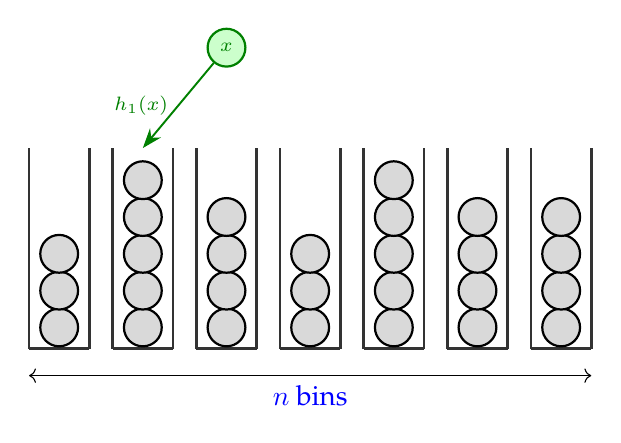
\begin{tikzpicture}[scale=0.85]
  % Dimensions matching Two-Choice Load Balancing slide
  \def\bw{0.9}
  \def\bh{3.0}
  \def\by{0}
  \def\bgap{0.35}
  \def\bs{0.48cm}
  \def\bsp{0.55}
  
  % Draw 7 rectangular bins
  \foreach \i in {0,...,6} {
    \pgfmathsetmacro{\xx}{\i*(\bw+\bgap)}
    \draw[line width=1pt, black!80] (\xx,\by) -- (\xx,\bh);
    \draw[line width=1pt, black!80] ({\xx+\bw},\by) -- ({\xx+\bw},\bh);
    \draw[line width=1pt, black!80] (\xx,\by) -- ({\xx+\bw},\by);
  }
  
  % Bin 0: 3 balls
  \foreach \j in {1,2,3} {
    \pgfmathsetmacro{\bx}{0*(\bw+\bgap)+0.5*\bw}
    \pgfmathsetmacro{\byy}{\by+0.32+(\j-1)*\bsp}
    \node[circle, draw, minimum size=\bs, inner sep=0pt, line width=0.8pt, fill=black!15] at (\bx,\byy) {};
  }
  % Bin 1: 5 balls
  \foreach \j in {1,2,3,4,5} {
    \pgfmathsetmacro{\bx}{1*(\bw+\bgap)+0.5*\bw}
    \pgfmathsetmacro{\byy}{\by+0.32+(\j-1)*\bsp}
    \node[circle, draw, minimum size=\bs, inner sep=0pt, line width=0.8pt, fill=black!15] at (\bx,\byy) {};
  }
  % Bin 2: 4 balls
  \foreach \j in {1,2,3,4} {
    \pgfmathsetmacro{\bx}{2*(\bw+\bgap)+0.5*\bw}
    \pgfmathsetmacro{\byy}{\by+0.32+(\j-1)*\bsp}
    \node[circle, draw, minimum size=\bs, inner sep=0pt, line width=0.8pt, fill=black!15] at (\bx,\byy) {};
  }
  % Bin 3: 3 balls
  \foreach \j in {1,2,3} {
    \pgfmathsetmacro{\bx}{3*(\bw+\bgap)+0.5*\bw}
    \pgfmathsetmacro{\byy}{\by+0.32+(\j-1)*\bsp}
    \node[circle, draw, minimum size=\bs, inner sep=0pt, line width=0.8pt, fill=black!15] at (\bx,\byy) {};
  }
  % Bin 4: 5 balls
  \foreach \j in {1,2,3,4,5} {
    \pgfmathsetmacro{\bx}{4*(\bw+\bgap)+0.5*\bw}
    \pgfmathsetmacro{\byy}{\by+0.32+(\j-1)*\bsp}
    \node[circle, draw, minimum size=\bs, inner sep=0pt, line width=0.8pt, fill=black!15] at (\bx,\byy) {};
  }
  % Bin 5: 4 balls
  \foreach \j in {1,2,3,4} {
    \pgfmathsetmacro{\bx}{5*(\bw+\bgap)+0.5*\bw}
    \pgfmathsetmacro{\byy}{\by+0.32+(\j-1)*\bsp}
    \node[circle, draw, minimum size=\bs, inner sep=0pt, line width=0.8pt, fill=black!15] at (\bx,\byy) {};
  }
  % Bin 6: 4 balls
  \foreach \j in {1,2,3,4} {
    \pgfmathsetmacro{\bx}{6*(\bw+\bgap)+0.5*\bw}
    \pgfmathsetmacro{\byy}{\by+0.32+(\j-1)*\bsp}
    \node[circle, draw, minimum size=\bs, inner sep=0pt, line width=0.8pt, fill=black!15] at (\bx,\byy) {};
  }
  
  % Ball x being inserted (green, centered between bins 1 and 3 like Two-Choice slide)
  \pgfmathsetmacro{\binoneX}{1*(\bw+\bgap)+0.5*\bw}
  \pgfmathsetmacro{\binthreeX}{3*(\bw+\bgap)+0.5*\bw}
  \pgfmathsetmacro{\xcenter}{(\binoneX+\binthreeX)/2}
  \node[circle, draw, minimum size=\bs, inner sep=0pt, line width=0.8pt, draw=green!50!black, fill=green!20, text=green!50!black] (xball) at (\xcenter,4.5) {\scriptsize $x$};
  
  % Single diagonal arrow to h_1(x) - pointing to bin 1
  \draw[-{Stealth[length=2.5mm, width=1.8mm]}, green!50!black, line width=0.7pt] (xball) -- (\binoneX,\bh) node[midway, left, green!50!black] {\scriptsize $h_1(x)$};
  
  % Label: n bins
  \pgfmathsetmacro{\totalw}{6*(\bw+\bgap)+\bw}
  \draw[<->] (0, -0.4) -- (\totalw, -0.4);
  \node[below, blue] at ({0.5*\totalw}, -0.4) {$n$ bins};
  
\end{tikzpicture}
\end{center}

\pause
\begin{itemize}
\item This is history-independent \hspace{0.3em}{\color{green!50!black}\ding{51}} \pause
\item The recourse is 0 \hspace{0.3em}{\color{green!50!black}\ding{51}} \pause
\item But... the overload is huge, roughly $\sqrt{m/n}$ \hspace{0.3em}{\color{red}\ding{55}}
\end{itemize}
\end{frame}

\begin{frame}{Baseline 2: Greedy Insertions}
  To insert a ball $x$, put it in the {\color{blue} emptier} of its choices:

\begin{center}
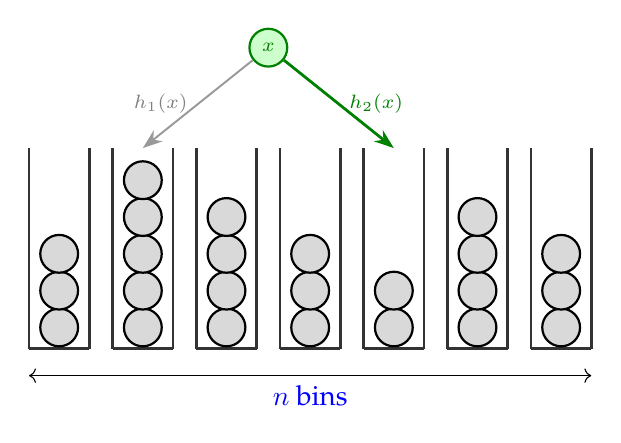
\begin{tikzpicture}[scale=0.85]
  % Dimensions matching Two-Choice Load Balancing slide
  \def\bw{0.9}
  \def\bh{3.0}
  \def\by{0}
  \def\bgap{0.35}
  \def\bs{0.48cm}
  \def\bsp{0.55}
  
  % Draw 7 rectangular bins
  \foreach \i in {0,...,6} {
    \pgfmathsetmacro{\xx}{\i*(\bw+\bgap)}
    \draw[line width=1pt, black!80] (\xx,\by) -- (\xx,\bh);
    \draw[line width=1pt, black!80] ({\xx+\bw},\by) -- ({\xx+\bw},\bh);
    \draw[line width=1pt, black!80] (\xx,\by) -- ({\xx+\bw},\by);
  }
  
  % Bin 0: 3 balls
  \foreach \j in {1,2,3} {
    \pgfmathsetmacro{\bx}{0*(\bw+\bgap)+0.5*\bw}
    \pgfmathsetmacro{\byy}{\by+0.32+(\j-1)*\bsp}
    \node[circle, draw, minimum size=\bs, inner sep=0pt, line width=0.8pt, fill=black!15] at (\bx,\byy) {};
  }
  % Bin 1: 5 balls (one of x's choices - fuller)
  \foreach \j in {1,2,3,4,5} {
    \pgfmathsetmacro{\bx}{1*(\bw+\bgap)+0.5*\bw}
    \pgfmathsetmacro{\byy}{\by+0.32+(\j-1)*\bsp}
    \node[circle, draw, minimum size=\bs, inner sep=0pt, line width=0.8pt, fill=black!15] at (\bx,\byy) {};
  }
  % Bin 2: 4 balls
  \foreach \j in {1,2,3,4} {
    \pgfmathsetmacro{\bx}{2*(\bw+\bgap)+0.5*\bw}
    \pgfmathsetmacro{\byy}{\by+0.32+(\j-1)*\bsp}
    \node[circle, draw, minimum size=\bs, inner sep=0pt, line width=0.8pt, fill=black!15] at (\bx,\byy) {};
  }
  % Bin 3: 3 balls
  \foreach \j in {1,2,3} {
    \pgfmathsetmacro{\bx}{3*(\bw+\bgap)+0.5*\bw}
    \pgfmathsetmacro{\byy}{\by+0.32+(\j-1)*\bsp}
    \node[circle, draw, minimum size=\bs, inner sep=0pt, line width=0.8pt, fill=black!15] at (\bx,\byy) {};
  }
  % Bin 4: 2 balls (one of x's choices - emptier, x goes here!)
  \foreach \j in {1,2} {
    \pgfmathsetmacro{\bx}{4*(\bw+\bgap)+0.5*\bw}
    \pgfmathsetmacro{\byy}{\by+0.32+(\j-1)*\bsp}
    \node[circle, draw, minimum size=\bs, inner sep=0pt, line width=0.8pt, fill=black!15] at (\bx,\byy) {};
  }
  % Bin 5: 4 balls
  \foreach \j in {1,2,3,4} {
    \pgfmathsetmacro{\bx}{5*(\bw+\bgap)+0.5*\bw}
    \pgfmathsetmacro{\byy}{\by+0.32+(\j-1)*\bsp}
    \node[circle, draw, minimum size=\bs, inner sep=0pt, line width=0.8pt, fill=black!15] at (\bx,\byy) {};
  }
  % Bin 6: 3 balls
  \foreach \j in {1,2,3} {
    \pgfmathsetmacro{\bx}{6*(\bw+\bgap)+0.5*\bw}
    \pgfmathsetmacro{\byy}{\by+0.32+(\j-1)*\bsp}
    \node[circle, draw, minimum size=\bs, inner sep=0pt, line width=0.8pt, fill=black!15] at (\bx,\byy) {};
  }
  
  % Ball x being inserted (green, centered between bins 1 and 4)
  \pgfmathsetmacro{\binoneX}{1*(\bw+\bgap)+0.5*\bw}
  \pgfmathsetmacro{\binfourX}{4*(\bw+\bgap)+0.5*\bw}
  \pgfmathsetmacro{\xcenter}{(\binoneX+\binfourX)/2}
  \node[circle, draw, minimum size=\bs, inner sep=0pt, line width=0.8pt, draw=green!50!black, fill=green!20, text=green!50!black] (xball) at (\xcenter,4.5) {\scriptsize $x$};
  
  % Two arrows to choices - bin 1 (fuller, grey) and bin 4 (emptier, blue/highlighted)
  \draw[-{Stealth[length=2.5mm, width=1.8mm]}, black!40, line width=0.7pt] (xball) -- (\binoneX,\bh) node[midway, left, black!50] {\scriptsize $h_1(x)$};
  \draw[-{Stealth[length=2.5mm, width=1.8mm]}, green!50!black, line width=1pt] (xball) -- (\binfourX,\bh) node[midway, right, green!50!black] {\scriptsize $h_2(x)$};
  
  % Label: n bins
  \pgfmathsetmacro{\totalw}{6*(\bw+\bgap)+\bw}
  \draw[<->] (0, -0.4) -- (\totalw, -0.4);
  \node[below, blue] at ({0.5*\totalw}, -0.4) {$n$ bins};
  
\end{tikzpicture}
\end{center}

\pause

  \begin{itemize}
  \item This is \textbf{not} history-independent  \hspace{0.3em}{\color{red}\ding{55}} \pause
  \item The recourse is 0 \hspace{0.3em}{\color{green!50!black}\ding{51}} \pause
  \item In the insertion-only case, the overload is $O(\log \log n)$ \hspace{0.3em}{\color{green!50!black}\ding{51}} \\
  {\hfill \color{gray} [Berenbrink, Czumaj, Steger, and V{\"o}cking '00]}
  \end{itemize}

  % \vspace{.4 cm}
  % \textbf{Interesting Fact: }In the dynamic case, overload remains open. \\
  % {\hfill \color{gray} [Bansal, Kuszmaul '22]}

\end{frame}

% OLD VERSION - COMMENTED OUT
% \begin{frame}{A Simple History-Independent Algorithm}\pause
% 
% \begin{center}
% \begin{tikzpicture}[scale=0.75]
%   % Dimensions matching Two-Choice Load Balancing slide
%   \def\bw{0.9}
%   \def\bh{3.0}
%   \def\by{0}
%   \def\bgap{0.35}
%   \def\bs{0.48cm}
%   \def\bsp{0.55}
%   
%   % Draw 7 rectangular bins
%   \foreach \i in {0,...,6} {
%     \pgfmathsetmacro{\xx}{\i*(\bw+\bgap)}
%     \draw[line width=1pt, black!80] (\xx,\by) -- (\xx,\bh);
%     \draw[line width=1pt, black!80] ({\xx+\bw},\by) -- ({\xx+\bw},\bh);
%     \draw[line width=1pt, black!80] (\xx,\by) -- ({\xx+\bw},\by);
%   }
%   
%   % Bin 0: 3 balls
%   \foreach \j in {1,2,3} {
%     \pgfmathsetmacro{\bx}{0*(\bw+\bgap)+0.5*\bw}
%     \pgfmathsetmacro{\byy}{\by+0.32+(\j-1)*\bsp}
%     \node[circle, draw, minimum size=\bs, inner sep=0pt, line width=0.8pt, fill=black!15] at (\bx,\byy) {};
%   }
%   % Bin 1: 5 balls (one of x's choices - fuller)
%   \foreach \j in {1,2,3,4,5} {
%     \pgfmathsetmacro{\bx}{1*(\bw+\bgap)+0.5*\bw}
%     \pgfmathsetmacro{\byy}{\by+0.32+(\j-1)*\bsp}
%     \node[circle, draw, minimum size=\bs, inner sep=0pt, line width=0.8pt, fill=black!15] at (\bx,\byy) {};
%   }
%   % Bin 2: 4 balls
%   \foreach \j in {1,2,3,4} {
%     \pgfmathsetmacro{\bx}{2*(\bw+\bgap)+0.5*\bw}
%     \pgfmathsetmacro{\byy}{\by+0.32+(\j-1)*\bsp}
%     \node[circle, draw, minimum size=\bs, inner sep=0pt, line width=0.8pt, fill=black!15] at (\bx,\byy) {};
%   }
%   % Bin 3: 3 balls
%   \foreach \j in {1,2,3} {
%     \pgfmathsetmacro{\bx}{3*(\bw+\bgap)+0.5*\bw}
%     \pgfmathsetmacro{\byy}{\by+0.32+(\j-1)*\bsp}
%     \node[circle, draw, minimum size=\bs, inner sep=0pt, line width=0.8pt, fill=black!15] at (\bx,\byy) {};
%   }
%   % Bin 4: 2 balls (one of x's choices - emptier, x goes here!)
%   \foreach \j in {1,2} {
%     \pgfmathsetmacro{\bx}{4*(\bw+\bgap)+0.5*\bw}
%     \pgfmathsetmacro{\byy}{\by+0.32+(\j-1)*\bsp}
%     \node[circle, draw, minimum size=\bs, inner sep=0pt, line width=0.8pt, fill=black!15] at (\bx,\byy) {};
%   }
%   % Bin 5: 4 balls
%   \foreach \j in {1,2,3,4} {
%     \pgfmathsetmacro{\bx}{5*(\bw+\bgap)+0.5*\bw}
%     \pgfmathsetmacro{\byy}{\by+0.32+(\j-1)*\bsp}
%     \node[circle, draw, minimum size=\bs, inner sep=0pt, line width=0.8pt, fill=black!15] at (\bx,\byy) {};
%   }
%   % Bin 6: 3 balls
%   \foreach \j in {1,2,3} {
%     \pgfmathsetmacro{\bx}{6*(\bw+\bgap)+0.5*\bw}
%     \pgfmathsetmacro{\byy}{\by+0.32+(\j-1)*\bsp}
%     \node[circle, draw, minimum size=\bs, inner sep=0pt, line width=0.8pt, fill=black!15] at (\bx,\byy) {};
%   }
%   
%   % Ball x being inserted (green, centered between bins 1 and 4)
%   \pgfmathsetmacro{\binoneX}{1*(\bw+\bgap)+0.5*\bw}
%   \pgfmathsetmacro{\binfourX}{4*(\bw+\bgap)+0.5*\bw}
%   \pgfmathsetmacro{\xcenter}{(\binoneX+\binfourX)/2}
%   \node[circle, draw, minimum size=\bs, inner sep=0pt, line width=0.8pt, draw=green!50!black, fill=green!20, text=green!50!black] (xball) at (\xcenter,4.5) {\scriptsize $x$};
%   
%   % Two arrows to choices - bin 1 (fuller, grey) and bin 4 (emptier, green/highlighted)
%   \draw[-{Stealth[length=2.5mm, width=1.8mm]}, black!40, line width=0.7pt] (xball) -- (\binoneX,\bh) node[midway, left, black!50] {\scriptsize $h_1(x)$};
%   \draw[-{Stealth[length=2.5mm, width=1.8mm]}, green!50!black, line width=1pt] (xball) -- (\binfourX,\bh) node[midway, right, green!50!black] {\scriptsize $h_2(x)$};
%   
%   % Label: n bins
%   \pgfmathsetmacro{\totalw}{6*(\bw+\bgap)+\bw}
%   \draw[<->] (0, -0.4) -- (\totalw, -0.4);
%   \node[below, blue] at ({0.5*\totalw}, -0.4) {$n$ bins};
%   
% \end{tikzpicture}
% \end{center}
% 
% \vspace{-0.2cm}
% Given a set $S$ of balls, define $\texttt{Greedy}(S)$ as:
% \begin{itemize}\setlength{\itemsep}{0pt}
% \item Start with empty bins.
% \item Sort the balls in $S$ to get a sequence $x_1, x_2, \ldots$.
% \item Insert $x_1, x_2, \ldots$ using the greedy algorithm. 
% \end{itemize} \pause
% 
% \vspace{.1 cm}
% 
% \textbf{A History-Independent Algorithm:} If $S$ is the current set, use $\texttt{Greedy}(S)$.
% 
% \end{frame}

\begin{frame}{Warmup: History-Independent Greedy}

\vspace{0.5cm}

\only<2->{%
\begin{center}
\begin{minipage}[b]{0.45\textwidth}
\centering
% Left picture: Current state A_S (appears on frame 2+)
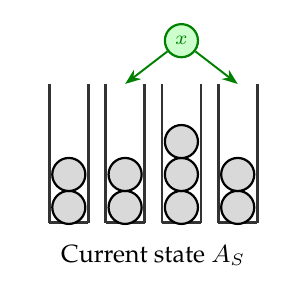
\begin{tikzpicture}[scale=0.55]
  \def\bw{0.9}
  \def\bh{3.2}
  \def\by{0}
  \def\bgap{0.4}
  \def\bs{0.42cm}
  \def\bsp{0.76}
  
  % Fixed bounding box
  \pgfmathsetmacro{\totalw}{3*(\bw+\bgap)+\bw}
  \path[use as bounding box] (-0.5, -0.7) rectangle ({\totalw+0.5}, 4.5);
  
  % Draw 4 rectangular bins
  \foreach \i in {0,...,3} {
    \pgfmathsetmacro{\xx}{\i*(\bw+\bgap)}
    \draw[line width=1pt, black!80] (\xx,\by) -- (\xx,\bh);
    \draw[line width=1pt, black!80] ({\xx+\bw},\by) -- ({\xx+\bw},\bh);
    \draw[line width=1pt, black!80] (\xx,\by) -- ({\xx+\bw},\by);
  }
  
  % Bin 0: 2 balls
  \foreach \j in {1,2} {
    \pgfmathsetmacro{\bx}{0*(\bw+\bgap)+0.5*\bw}
    \pgfmathsetmacro{\byy}{\by+0.35+(\j-1)*\bsp}
    \node[circle, draw, minimum size=\bs, inner sep=0pt, line width=0.8pt, fill=black!15] at (\bx,\byy) {};
  }
  % Bin 1: 2 balls
  \foreach \j in {1,2} {
    \pgfmathsetmacro{\bx}{1*(\bw+\bgap)+0.5*\bw}
    \pgfmathsetmacro{\byy}{\by+0.35+(\j-1)*\bsp}
    \node[circle, draw, minimum size=\bs, inner sep=0pt, line width=0.8pt, fill=black!15] at (\bx,\byy) {};
  }
  % Bin 2: 3 balls
  \foreach \j in {1,2,3} {
    \pgfmathsetmacro{\bx}{2*(\bw+\bgap)+0.5*\bw}
    \pgfmathsetmacro{\byy}{\by+0.35+(\j-1)*\bsp}
    \node[circle, draw, minimum size=\bs, inner sep=0pt, line width=0.8pt, fill=black!15] at (\bx,\byy) {};
  }
  % Bin 3: 2 balls
  \foreach \j in {1,2} {
    \pgfmathsetmacro{\bx}{3*(\bw+\bgap)+0.5*\bw}
    \pgfmathsetmacro{\byy}{\by+0.35+(\j-1)*\bsp}
    \node[circle, draw, minimum size=\bs, inner sep=0pt, line width=0.8pt, fill=black!15] at (\bx,\byy) {};
  }
  
  % Ball x being inserted (green, between bins 1 and 3)
  \pgfmathsetmacro{\binoneX}{1*(\bw+\bgap)+0.5*\bw}
  \pgfmathsetmacro{\binthreeX}{3*(\bw+\bgap)+0.5*\bw}
  \pgfmathsetmacro{\xcenter}{(\binoneX+\binthreeX)/2}
  \node[circle, draw, minimum size=\bs, inner sep=0pt, line width=0.8pt, draw=green!50!black, fill=green!20, text=green!50!black] (xball) at (\xcenter,4.2) {\scriptsize $x$};
  
  % Arrows to two choices (bins 1 and 3)
  \draw[-{Stealth[length=2mm, width=1.5mm]}, green!50!black, line width=0.7pt] (xball) -- (\binoneX,\bh);
  \draw[-{Stealth[length=2mm, width=1.5mm]}, green!50!black, line width=0.7pt] (xball) -- (\binthreeX,\bh);
  
  % Label below
  \pgfmathsetmacro{\totalw}{3*(\bw+\bgap)+\bw}
  \node[below] at ({0.5*\totalw}, -0.3) {\small Current state $A_S$};
  
\end{tikzpicture}%
\end{minipage}%
\hfill%
\raisebox{0.8cm}{\Large $\longrightarrow$}%
\hfill%
\begin{minipage}[b]{0.45\textwidth}
\centering
% Right picture: Computing A_{S∪x} with animation
\begin{tikzpicture}[scale=0.55]
  \def\bw{0.9}
  \def\bh{3.2}
  \def\by{0}
  \def\bgap{0.4}
  \def\bs{0.42cm}
  \def\bsp{0.76}
  
  % Fixed bounding box
  \pgfmathsetmacro{\totalw}{3*(\bw+\bgap)+\bw}
  \path[use as bounding box] (-0.5, -0.7) rectangle ({\totalw+0.5}, 4.5);
  
  % Draw 4 rectangular bins (always visible)
  \foreach \i in {0,...,3} {
    \pgfmathsetmacro{\xx}{\i*(\bw+\bgap)}
    \draw[line width=1pt, black!80] (\xx,\by) -- (\xx,\bh);
    \draw[line width=1pt, black!80] ({\xx+\bw},\by) -- ({\xx+\bw},\bh);
    \draw[line width=1pt, black!80] (\xx,\by) -- ({\xx+\bw},\by);
  }
  
  % Frame 4: Row of 10 balls above bins (9 grey + 1 green as 5th ball)
  \only<4>{
    \foreach \i in {0,...,9} {
      \pgfmathsetmacro{\ballx}{\i*0.76 - 1.0}
      \ifnum\i=4
        \node[circle, draw, minimum size=\bs, inner sep=0pt, line width=0.8pt, draw=green!50!black, fill=green!20, overlay] at (\ballx, 4.0) {};
      \else
        \node[circle, draw, minimum size=\bs, inner sep=0pt, line width=0.8pt, fill=black!15, overlay] at (\ballx, 4.0) {};
      \fi
    }
  }
  
  % Frame 5+: Balls in bins (greedy assignment) - 10 balls total, loads 2,3,3,2 with green in bin 3
  \only<5->{
    % Bin 0: 2 balls (grey)
    \foreach \j in {1,2} {
      \pgfmathsetmacro{\bx}{0*(\bw+\bgap)+0.5*\bw}
      \pgfmathsetmacro{\byy}{\by+0.35+(\j-1)*\bsp}
      \node[circle, draw, minimum size=\bs, inner sep=0pt, line width=0.8pt, fill=black!15] at (\bx,\byy) {};
    }
    % Bin 1: 3 balls (grey)
    \foreach \j in {1,2,3} {
      \pgfmathsetmacro{\bx}{1*(\bw+\bgap)+0.5*\bw}
      \pgfmathsetmacro{\byy}{\by+0.35+(\j-1)*\bsp}
      \node[circle, draw, minimum size=\bs, inner sep=0pt, line width=0.8pt, fill=black!15] at (\bx,\byy) {};
    }
    % Bin 2: 3 balls (grey)
    \foreach \j in {1,2,3} {
      \pgfmathsetmacro{\bx}{2*(\bw+\bgap)+0.5*\bw}
      \pgfmathsetmacro{\byy}{\by+0.35+(\j-1)*\bsp}
      \node[circle, draw, minimum size=\bs, inner sep=0pt, line width=0.8pt, fill=black!15] at (\bx,\byy) {};
    }
    % Bin 3: 1 grey + 1 green on top (2 total)
    \pgfmathsetmacro{\bx}{3*(\bw+\bgap)+0.5*\bw}
    \pgfmathsetmacro{\byy}{\by+0.35}
    \node[circle, draw, minimum size=\bs, inner sep=0pt, line width=0.8pt, fill=black!15] at (\bx,\byy) {};
    \pgfmathsetmacro{\byy}{\by+0.35+\bsp}
    \node[circle, draw, minimum size=\bs, inner sep=0pt, line width=0.8pt, draw=green!50!black, fill=green!20] at (\bx,\byy) {};
  }
  
  % Label below
  \pgfmathsetmacro{\totalw}{3*(\bw+\bgap)+\bw}
  \node[below] at ({0.5*\totalw}, -0.3) {\small Computing $A_{S \cup \{x\}}$};
  
\end{tikzpicture}%
\end{minipage}
\end{center}
}% end of only<2->

\vfill
\vspace{0.5cm}

% Text area with the greedy simulation steps (appears on frame 3+)
\only<3->{%
To compute $A_{S \cup \{x\}}$:
\begin{enumerate}\setlength{\itemsep}{0pt}
\item Empty out the bins.
\item Sort the balls in $S \cup \{x\}$ to get $x_1, x_2, \ldots$
\item Insert the balls in sorted order using greedy.
\end{enumerate}
}%

\end{frame}

\begin{frame}{Analyzing History-Independent Greedy}

\begin{center}
\begin{minipage}[b]{0.45\textwidth}
\centering
% Left picture: Current state A_S
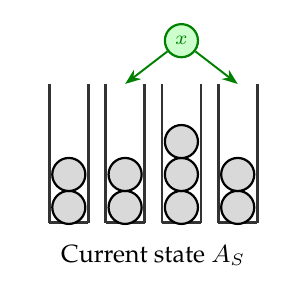
\begin{tikzpicture}[scale=0.55]
  \def\bw{0.9}
  \def\bh{3.2}
  \def\by{0}
  \def\bgap{0.4}
  \def\bs{0.42cm}
  \def\bsp{0.76}
  
  % Fixed bounding box
  \pgfmathsetmacro{\totalw}{3*(\bw+\bgap)+\bw}
  \path[use as bounding box] (-0.5, -0.7) rectangle ({\totalw+0.5}, 4.5);
  
  % Draw 4 rectangular bins
  \foreach \i in {0,...,3} {
    \pgfmathsetmacro{\xx}{\i*(\bw+\bgap)}
    \draw[line width=1pt, black!80] (\xx,\by) -- (\xx,\bh);
    \draw[line width=1pt, black!80] ({\xx+\bw},\by) -- ({\xx+\bw},\bh);
    \draw[line width=1pt, black!80] (\xx,\by) -- ({\xx+\bw},\by);
  }
  
  % Bin 0: 2 balls
  \foreach \j in {1,2} {
    \pgfmathsetmacro{\bx}{0*(\bw+\bgap)+0.5*\bw}
    \pgfmathsetmacro{\byy}{\by+0.35+(\j-1)*\bsp}
    \node[circle, draw, minimum size=\bs, inner sep=0pt, line width=0.8pt, fill=black!15] at (\bx,\byy) {};
  }
  % Bin 1: 2 balls
  \foreach \j in {1,2} {
    \pgfmathsetmacro{\bx}{1*(\bw+\bgap)+0.5*\bw}
    \pgfmathsetmacro{\byy}{\by+0.35+(\j-1)*\bsp}
    \node[circle, draw, minimum size=\bs, inner sep=0pt, line width=0.8pt, fill=black!15] at (\bx,\byy) {};
  }
  % Bin 2: 3 balls
  \foreach \j in {1,2,3} {
    \pgfmathsetmacro{\bx}{2*(\bw+\bgap)+0.5*\bw}
    \pgfmathsetmacro{\byy}{\by+0.35+(\j-1)*\bsp}
    \node[circle, draw, minimum size=\bs, inner sep=0pt, line width=0.8pt, fill=black!15] at (\bx,\byy) {};
  }
  % Bin 3: 2 balls
  \foreach \j in {1,2} {
    \pgfmathsetmacro{\bx}{3*(\bw+\bgap)+0.5*\bw}
    \pgfmathsetmacro{\byy}{\by+0.35+(\j-1)*\bsp}
    \node[circle, draw, minimum size=\bs, inner sep=0pt, line width=0.8pt, fill=black!15] at (\bx,\byy) {};
  }
  
  % Ball x being inserted (green, between bins 1 and 3)
  \pgfmathsetmacro{\binoneX}{1*(\bw+\bgap)+0.5*\bw}
  \pgfmathsetmacro{\binthreeX}{3*(\bw+\bgap)+0.5*\bw}
  \pgfmathsetmacro{\xcenter}{(\binoneX+\binthreeX)/2}
  \node[circle, draw, minimum size=\bs, inner sep=0pt, line width=0.8pt, draw=green!50!black, fill=green!20, text=green!50!black] (xball) at (\xcenter,4.2) {\scriptsize $x$};
  
  % Arrows to two choices (bins 1 and 3)
  \draw[-{Stealth[length=2mm, width=1.5mm]}, green!50!black, line width=0.7pt] (xball) -- (\binoneX,\bh);
  \draw[-{Stealth[length=2mm, width=1.5mm]}, green!50!black, line width=0.7pt] (xball) -- (\binthreeX,\bh);
  
  % Label below
  \node[below] at ({0.5*\totalw}, -0.3) {\small Current state $A_S$};
  
\end{tikzpicture}%
\end{minipage}%
\hfill%
\raisebox{0.8cm}{\Large $\longrightarrow$}%
\hfill%
\begin{minipage}[b]{0.45\textwidth}
\centering
% Right picture: Computing A_{S∪x} with balls in bins
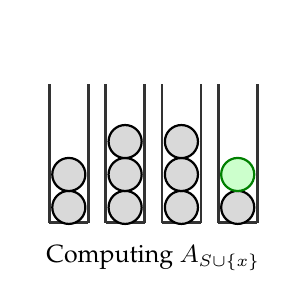
\begin{tikzpicture}[scale=0.55]
  \def\bw{0.9}
  \def\bh{3.2}
  \def\by{0}
  \def\bgap{0.4}
  \def\bs{0.42cm}
  \def\bsp{0.76}
  
  % Fixed bounding box
  \pgfmathsetmacro{\totalw}{3*(\bw+\bgap)+\bw}
  \path[use as bounding box] (-0.5, -0.7) rectangle ({\totalw+0.5}, 4.5);
  
  % Draw 4 rectangular bins
  \foreach \i in {0,...,3} {
    \pgfmathsetmacro{\xx}{\i*(\bw+\bgap)}
    \draw[line width=1pt, black!80] (\xx,\by) -- (\xx,\bh);
    \draw[line width=1pt, black!80] ({\xx+\bw},\by) -- ({\xx+\bw},\bh);
    \draw[line width=1pt, black!80] (\xx,\by) -- ({\xx+\bw},\by);
  }
  
  % Bin 0: 2 balls (grey)
  \foreach \j in {1,2} {
    \pgfmathsetmacro{\bx}{0*(\bw+\bgap)+0.5*\bw}
    \pgfmathsetmacro{\byy}{\by+0.35+(\j-1)*\bsp}
    \node[circle, draw, minimum size=\bs, inner sep=0pt, line width=0.8pt, fill=black!15] at (\bx,\byy) {};
  }
  % Bin 1: 3 balls (grey)
  \foreach \j in {1,2,3} {
    \pgfmathsetmacro{\bx}{1*(\bw+\bgap)+0.5*\bw}
    \pgfmathsetmacro{\byy}{\by+0.35+(\j-1)*\bsp}
    \node[circle, draw, minimum size=\bs, inner sep=0pt, line width=0.8pt, fill=black!15] at (\bx,\byy) {};
  }
  % Bin 2: 3 balls (grey)
  \foreach \j in {1,2,3} {
    \pgfmathsetmacro{\bx}{2*(\bw+\bgap)+0.5*\bw}
    \pgfmathsetmacro{\byy}{\by+0.35+(\j-1)*\bsp}
    \node[circle, draw, minimum size=\bs, inner sep=0pt, line width=0.8pt, fill=black!15] at (\bx,\byy) {};
  }
  % Bin 3: 1 grey + 1 green on top (2 total)
  \pgfmathsetmacro{\bx}{3*(\bw+\bgap)+0.5*\bw}
  \pgfmathsetmacro{\byy}{\by+0.35}
  \node[circle, draw, minimum size=\bs, inner sep=0pt, line width=0.8pt, fill=black!15] at (\bx,\byy) {};
  \pgfmathsetmacro{\byy}{\by+0.35+\bsp}
  \node[circle, draw, minimum size=\bs, inner sep=0pt, line width=0.8pt, draw=green!50!black, fill=green!20] at (\bx,\byy) {};
  
  % Label below
  \node[below] at ({0.5*\totalw}, -0.3) {\small Computing $A_{S \cup \{x\}}$};
  
\end{tikzpicture}%
\end{minipage}
\end{center}

    \pause
    \begin{itemize}
    \item The algorithm is history independent \hspace{0.3em}{\color{green!50!black}\ding{51}}  \pause 
    \item The overload is $O(\log \log n)$ \hspace{0.3em}{\color{green!50!black}\ding{51}} \pause 
    \item What is the recourse?
    \end{itemize}
\end{frame}


% ============== Two-World Slides ==============

% --- Frame 10 (PDF p10): initial two worlds, empty bins ---
\begin{frame}{Analyzing the Recourse}
\TopSeq
\TwoWorldFigure{ }{ }
\vfill
How many balls change assignments between $A_S$ and $A_{S \cup \{x\}}$?
\end{frame}

% --- Frame 12 (PDF p12): x1 chooses among 2 bins ---
\begin{frame}{Analyzing the Recourse}
\TopSeq
\TwoWorldFigure{
  \node[circle,draw,minimum size=0.55cm,inner sep=0pt,RedBallStyle] (aL) at (-3.825,1.5) {$x_1$};
  \foreach \b in {1,3}{\draw[-{Stealth[length=2.5mm, width=1.8mm]},black!50,line width=0.7pt] (aL) -- (LT\b);}
}{
  \node[circle,draw,minimum size=0.55cm,inner sep=0pt,RedBallStyle] (aR) at (2.575,1.5) {$x_1$};
  \foreach \b in {1,3}{\draw[-{Stealth[length=2.5mm, width=1.8mm]},black!50,line width=0.7pt] (aR) -- (RT\b);}
}
\vfill
\hspace*{-1cm}\parbox{\dimexpr\textwidth+1cm}{%
% \begin{itemize}
% \item Two identical worlds, same insertion sequence
% \item World 1 will later receive one extra ball $x$
% \end{itemize}
}
\end{frame}

% --- Frame 13 (PDF p13): x1 placed in bin 1 (both worlds) ---
\begin{frame}{Analyzing the Recourse}
\TopSeq
\TwoWorldFigure{
  \BallInBin{\xL}{1}{1}{RedBallStyle}{$x_1$}
}{
  \BallInBin{\xR}{1}{1}{RedBallStyle}{$x_1$}
}
\vfill
\hspace*{-1cm}\parbox{\dimexpr\textwidth+1cm}{%
% \begin{itemize}
% \item Two identical worlds, same insertion sequence
% \item World 1 will later receive one extra ball $x$
% \end{itemize}
}
\end{frame}

% --- Frame 15 (PDF p15): x2 chooses among 2 bins (1 and 2) ---
\begin{frame}{Analyzing the Recourse}
\TopSeq
\TwoWorldFigure{
  \BallInBin{\xL}{1}{1}{}{}
  \node[circle,draw,minimum size=0.55cm,inner sep=0pt,RedBallStyle] (aL) at (-4.45,1.5) {$x_2$};
  \foreach \b in {1,2}{\draw[-{Stealth[length=2.5mm, width=1.8mm]},black!50,line width=0.7pt] (aL) -- (LT\b);}
}{
  \BallInBin{\xR}{1}{1}{}{}
  \node[circle,draw,minimum size=0.55cm,inner sep=0pt,RedBallStyle] (aR) at (1.95,1.5) {$x_2$};
  \foreach \b in {1,2}{\draw[-{Stealth[length=2.5mm, width=1.8mm]},black!50,line width=0.7pt] (aR) -- (RT\b);}
}
\vfill
\hspace*{-1cm}\parbox{\dimexpr\textwidth+1cm}{%
% \begin{itemize}
% \item Two identical worlds, same insertion sequence
% \item World 1 will later receive one extra ball $x$
% \end{itemize}
}
\end{frame}

% --- Frame 16 (PDF p16): x2 placed in bin 2 (both worlds), plus prior ball in bin1 ---
\begin{frame}{Analyzing the Recourse}
\TopSeq
\TwoWorldFigure{
  \BallInBin{\xL}{1}{1}{}{}
  \BallInBin{\xL}{2}{1}{RedBallStyle}{$x_2$}
}{
  \BallInBin{\xR}{1}{1}{}{}
  \BallInBin{\xR}{2}{1}{RedBallStyle}{$x_2$}
}
\vfill
\hspace*{-1cm}\parbox{\dimexpr\textwidth+1cm}{%
% \begin{itemize}
% \item Two identical worlds, same insertion sequence
% \item World 1 will later receive one extra ball $x$
% \end{itemize}
}
\end{frame}

% --- Frame 18 (PDF p18): x3 chooses among 2 bins (1 and 2) ---
\begin{frame}{Analyzing the Recourse}
\TopSeq
\TwoWorldFigure{
  \BallInBin{\xL}{1}{1}{}{}
  \BallInBin{\xL}{2}{1}{}{}
  \node[circle,draw,minimum size=0.55cm,inner sep=0pt,RedBallStyle] (aL) at (-4.45,1.5) {$x_3$};
  \foreach \b in {1,2}{\draw[-{Stealth[length=2.5mm, width=1.8mm]},black!50,line width=0.7pt] (aL) -- (LT\b);}
}{
  \BallInBin{\xR}{1}{1}{}{}
  \BallInBin{\xR}{2}{1}{}{}
  \node[circle,draw,minimum size=0.55cm,inner sep=0pt,RedBallStyle] (aR) at (1.95,1.5) {$x_3$};
  \foreach \b in {1,2}{\draw[-{Stealth[length=2.5mm, width=1.8mm]},black!50,line width=0.7pt] (aR) -- (RT\b);}
}
\vfill
\hspace*{-1cm}\parbox{\dimexpr\textwidth+1cm}{%
% \begin{itemize}
% \item Two identical worlds, same insertion sequence
% \item World 1 will later receive one extra ball $x$
% \end{itemize}
}
\end{frame}

% --- Frame 19 (PDF p19): x3 placed in both worlds ---
\begin{frame}{Analyzing the Recourse}
\TopSeq
\TwoWorldFigure{
  \BallInBin{\xL}{1}{1}{}{}
  \BallInBin{\xL}{2}{1}{}{}
  \BallInBin{\xL}{2}{2}{RedBallStyle}{$x_3$}
}{
  \BallInBin{\xR}{1}{1}{}{}
  \BallInBin{\xR}{2}{1}{}{}
  \BallInBin{\xR}{2}{2}{RedBallStyle}{$x_3$}
}
\vfill
\hspace*{-1cm}\parbox{\dimexpr\textwidth+1cm}{%
% \begin{itemize}
% \item Two identical worlds, same insertion sequence
% \item World 1 will later receive one extra ball $x$
% \end{itemize}
}
\end{frame}

% --- Frame 21 (PDF p21): x4 chooses among 2 bins (2 and 4) in both worlds ---
\begin{frame}{Analyzing the Recourse}
\TopSeq
\TwoWorldFigure{
  \BallInBin{\xL}{1}{1}{}{}
  \BallInBin{\xL}{2}{1}{}{}
  \BallInBin{\xL}{2}{2}{}{}
  \node[circle,draw,minimum size=0.55cm,inner sep=0pt,RedBallStyle] (aL) at (-2.575,1.5) {$x_4$};
  \foreach \b in {2,4}{\draw[-{Stealth[length=2.5mm, width=1.8mm]},black!50,line width=0.7pt] (aL) -- (LT\b);}
}{
  \BallInBin{\xR}{1}{1}{}{}
  \BallInBin{\xR}{2}{1}{}{}
  \BallInBin{\xR}{2}{2}{}{}
  \node[circle,draw,minimum size=0.55cm,inner sep=0pt,RedBallStyle] (aR) at (3.825,1.5) {$x_4$};
  \foreach \b in {2,4}{\draw[-{Stealth[length=2.5mm, width=1.8mm]},black!50,line width=0.7pt] (aR) -- (RT\b);}
}
\vfill
\hspace*{-1cm}\parbox{\dimexpr\textwidth+1cm}{%
% \begin{itemize}
% \item Two identical worlds, same insertion sequence
% \item World 1 will later receive one extra ball $x$
% \end{itemize}
}
\end{frame}

% --- Frame 22 (PDF p22): x4 placed in bin4 in both worlds ---
\begin{frame}{Analyzing the Recourse}
\TopSeq
\TwoWorldFigure{
  \BallInBin{\xL}{1}{1}{}{}
  \BallInBin{\xL}{2}{1}{}{}
  \BallInBin{\xL}{2}{2}{}{}
  \BallInBin{\xL}{4}{1}{RedBallStyle}{$x_4$}
}{
  \BallInBin{\xR}{1}{1}{}{}
  \BallInBin{\xR}{2}{1}{}{}
  \BallInBin{\xR}{2}{2}{}{}
  \BallInBin{\xR}{4}{1}{RedBallStyle}{$x_4$}
}
\vfill
\hspace*{-1cm}\parbox{\dimexpr\textwidth+1cm}{%
% \begin{itemize}
% \item Two identical worlds, same insertion sequence
% \item World 1 will later receive one extra ball $x$
% \end{itemize}
}
\end{frame}

% --- Frame 24 (PDF p24): x* (blue outline) chooses between bins (3 and 4) in world1 ---
\begin{frame}{Analyzing the Recourse}
\TopSeq
\TwoWorldFigure{
  \BallInBin{\xL}{1}{1}{}{}
  \BallInBin{\xL}{2}{1}{}{}
  \BallInBin{\xL}{2}{2}{}{}
  \BallInBin{\xL}{4}{1}{}{}
}{
  \BallInBin{\xR}{1}{1}{}{}
  \BallInBin{\xR}{2}{1}{}{}
  \BallInBin{\xR}{2}{2}{}{}
  \BallInBin{\xR}{4}{1}{}{}
  \node[circle,draw,minimum size=0.55cm,inner sep=0pt,BlueOutlineStyle] (bR) at (3.825,1.5) {$x$};
  \foreach \bb in {2,4}{\draw[-{Stealth[length=2.5mm, width=1.8mm]},green!50!black,line width=0.7pt] (bR) -- (RT\bb);}
}
\vfill
\hspace*{-1cm}\parbox{\dimexpr\textwidth+1cm}{%
% \begin{itemize}
% \item $x$ arrives only in World 1
% \end{itemize}
}
\end{frame}

% --- Frame 25 (PDF p25): x* placed (blue outline, labeled) in world1 bin4 top ---
\begin{frame}{Analyzing the Recourse}
\TopSeq
\TwoWorldFigure{
  \BallInBin{\xL}{1}{1}{}{}
  \BallInBin{\xL}{2}{1}{}{}
  \BallInBin{\xL}{2}{2}{}{}
  \BallInBin{\xL}{4}{1}{}{}
}{
  \BallInBin{\xR}{1}{1}{}{}
  \BallInBin{\xR}{2}{1}{}{}
  \BallInBin{\xR}{2}{2}{}{}
  \BallInBin{\xR}{4}{1}{}{}
  \BallInBin{\xR}{4}{2}{BlueOutlineStyle}{$x$}
}
\vfill
\hspace*{-1cm}\parbox{\dimexpr\textwidth+1cm}{%
% \begin{itemize}
% \item $x$ arrives only in World 1
% \end{itemize}
}
\end{frame}

% --- Frame 26: Question about divergence ---
% \begin{frame}{Analyzing the Recourse}
% \TopSeq
% \TwoWorldFigure{
%   \BallInBin{\xL}{1}{1}{}{}
%   \BallInBin{\xL}{2}{1}{}{}
%   \BallInBin{\xL}{2}{2}{}{}
%   \BallInBin{\xL}{4}{1}{}{}
% }{
%   \BallInBin{\xR}{1}{1}{}{}
%   \BallInBin{\xR}{2}{1}{}{}
%   \BallInBin{\xR}{2}{2}{}{}
%   \BallInBin{\xR}{4}{1}{}{}
%   \BallInBin{\xR}{4}{2}{BlueFillStyle}{}
% }
% \vfill
% \hspace*{-0.5cm}\parbox{\dimexpr\textwidth+0.5cm}{%
% % \textbf{Question:} How do subsequent insertions differ between the two worlds?
% }
% \end{frame}

% --- Frame 27 (PDF p27): future insertions: option 1 (No recourse) ---
\begin{frame}{Analyzing the Recourse}
\TopSeq
\TwoWorldFigure{
  \BallInBin{\xL}{1}{1}{}{}
  \BallInBin{\xL}{2}{1}{}{}
  \BallInBin{\xL}{2}{2}{}{}
  \BallInBin{\xL}{4}{1}{}{}
}{
  \BallInBin{\xR}{1}{1}{}{}
  \BallInBin{\xR}{2}{1}{}{}
  \BallInBin{\xR}{2}{2}{}{}
  \BallInBin{\xR}{4}{1}{}{}
  \BallInBin{\xR}{4}{2}{BlueFillStyle}{}
}

\vspace{.2 cm}

\hspace*{-0.5cm}\parbox{\dimexpr\textwidth+0.5cm}{%
Subsequent balls will experience either: \pause
\begin{enumerate}
\item No recourse
\end{enumerate}
}
\end{frame}

% --- Frame 28 (PDF p28): x5 chooses among 2 bins (1 and 3) ---
\begin{frame}{Analyzing the Recourse}
\TopSeq
\TwoWorldFigure{
  \BallInBin{\xL}{1}{1}{}{}
  \BallInBin{\xL}{2}{1}{}{}
  \BallInBin{\xL}{2}{2}{}{}
  \BallInBin{\xL}{4}{1}{}{}
  \node[circle,draw,minimum size=0.55cm,inner sep=0pt,RedBallStyle] (aL) at (-3.825,1.5) {$x_5$};
  \foreach \b in {1,3}{\draw[-{Stealth[length=2.5mm, width=1.8mm]},black!50,line width=0.7pt] (aL) -- (LT\b);}
}{
  \BallInBin{\xR}{1}{1}{}{}
  \BallInBin{\xR}{2}{1}{}{}
  \BallInBin{\xR}{2}{2}{}{}
  \BallInBin{\xR}{4}{1}{}{}
  \BallInBin{\xR}{4}{2}{BlueFillStyle}{}
  \node[circle,draw,minimum size=0.55cm,inner sep=0pt,RedBallStyle] (aR) at (2.575,1.5) {$x_5$};
  \foreach \b in {1,3}{\draw[-{Stealth[length=2.5mm, width=1.8mm]},black!50,line width=0.7pt] (aR) -- (RT\b);}
}

\vspace{.2 cm}

\hspace*{-0.5cm}\parbox{\dimexpr\textwidth+0.5cm}{%
Future insertions will experience either:
\begin{enumerate}
\item No recourse
\end{enumerate}
}
\end{frame}

% --- Frame 29 (PDF p29): x5 placed in bin3 (both worlds) ---
\begin{frame}{Analyzing the Recourse}
\TopSeq
\TwoWorldFigure{
  \BallInBin{\xL}{1}{1}{}{}
  \BallInBin{\xL}{2}{1}{}{}
  \BallInBin{\xL}{2}{2}{}{}
  \BallInBin{\xL}{3}{1}{RedBallStyle}{$x_5$}
  \BallInBin{\xL}{4}{1}{}{}
}{
  \BallInBin{\xR}{1}{1}{}{}
  \BallInBin{\xR}{2}{1}{}{}
  \BallInBin{\xR}{2}{2}{}{}
  \BallInBin{\xR}{3}{1}{RedBallStyle}{$x_5$}
  \BallInBin{\xR}{4}{1}{}{}
  \BallInBin{\xR}{4}{2}{BlueFillStyle}{}
}

\vspace{.2 cm}

\hspace*{-0.5cm}\parbox{\dimexpr\textwidth+0.5cm}{%
Subsequent balls will experience either:
\begin{enumerate}
\item No recourse
\end{enumerate}
}
\end{frame}

% --- Frame 31 (PDF p31): x6 chooses among 2 bins (1 and 3) ---
\begin{frame}{Analyzing the Recourse}
\TopSeq
\TwoWorldFigure{
  \BallInBin{\xL}{1}{1}{}{}
  \BallInBin{\xL}{2}{1}{}{}
  \BallInBin{\xL}{2}{2}{}{}
  \BallInBin{\xL}{3}{1}{}{}
  \BallInBin{\xL}{4}{1}{}{}
  \node[circle,draw,minimum size=0.55cm,inner sep=0pt,RedBallStyle] (aL) at (-3.825,1.5) {$x_6$};
  \foreach \b in {1,3}{\draw[-{Stealth[length=2.5mm, width=1.8mm]},black!50,line width=0.7pt] (aL) -- (LT\b);}
}{
  \BallInBin{\xR}{1}{1}{}{}
  \BallInBin{\xR}{2}{1}{}{}
  \BallInBin{\xR}{2}{2}{}{}
  \BallInBin{\xR}{3}{1}{}{}
  \BallInBin{\xR}{4}{1}{}{}
  \BallInBin{\xR}{4}{2}{BlueFillStyle}{}
  \node[circle,draw,minimum size=0.55cm,inner sep=0pt,RedBallStyle] (aR) at (2.575,1.5) {$x_6$};
  \foreach \b in {1,3}{\draw[-{Stealth[length=2.5mm, width=1.8mm]},black!50,line width=0.7pt] (aR) -- (RT\b);}
}

\vspace{.2 cm}

\hspace*{-0.5cm}\parbox{\dimexpr\textwidth+0.5cm}{%
Subsequent balls will experience either:
\begin{enumerate}
\item No recourse
\end{enumerate}
}
\end{frame}

% --- Frame 32 (PDF p32): x6 placed in bin3 (level 2) ---
\begin{frame}{Analyzing the Recourse}
\TopSeq
\TwoWorldFigure{
  \BallInBin{\xL}{1}{1}{}{}
  \BallInBin{\xL}{2}{1}{}{}
  \BallInBin{\xL}{2}{2}{}{}
  \BallInBin{\xL}{3}{1}{}{}
  \BallInBin{\xL}{3}{2}{RedBallStyle}{$x_6$}
  \BallInBin{\xL}{4}{1}{}{}
}{
  \BallInBin{\xR}{1}{1}{}{}
  \BallInBin{\xR}{2}{1}{}{}
  \BallInBin{\xR}{2}{2}{}{}
  \BallInBin{\xR}{3}{1}{}{}
  \BallInBin{\xR}{3}{2}{RedBallStyle}{$x_6$}
  \BallInBin{\xR}{4}{1}{}{}
  \BallInBin{\xR}{4}{2}{BlueFillStyle}{}
}
\vfill
\hspace*{-0.5cm}\parbox{\dimexpr\textwidth+0.5cm}{%
Subsequent balls will experience either:
\begin{enumerate}
\item No recourse
\end{enumerate}
}
\end{frame}

% --- Frame 34 (PDF p34): x7 chooses among 2 bins (2 and 3) ---
\begin{frame}{Analyzing the Recourse}
\TopSeq
\TwoWorldFigure{
  \BallInBin{\xL}{1}{1}{}{}
  \BallInBin{\xL}{2}{1}{}{}
  \BallInBin{\xL}{2}{2}{}{}
  \BallInBin{\xL}{3}{1}{}{}
  \BallInBin{\xL}{3}{2}{}{}
  \BallInBin{\xL}{4}{1}{}{}
  \node[circle,draw,minimum size=0.55cm,inner sep=0pt,RedBallStyle] (aL) at (-3.2,1.5) {$x_7$};
  \foreach \b in {2,3}{\draw[-{Stealth[length=2.5mm, width=1.8mm]},black!50,line width=0.7pt] (aL) -- (LT\b);}
}{
  \BallInBin{\xR}{1}{1}{}{}
  \BallInBin{\xR}{2}{1}{}{}
  \BallInBin{\xR}{2}{2}{}{}
  \BallInBin{\xR}{3}{1}{}{}
  \BallInBin{\xR}{3}{2}{}{}
  \BallInBin{\xR}{4}{1}{}{}
  \BallInBin{\xR}{4}{2}{BlueFillStyle}{}
  \node[circle,draw,minimum size=0.55cm,inner sep=0pt,RedBallStyle] (aR) at (3.2,1.5) {$x_7$};
  \foreach \b in {2,3}{\draw[-{Stealth[length=2.5mm, width=1.8mm]},black!50,line width=0.7pt] (aR) -- (RT\b);}
}

\vspace{.2 cm}

\hspace*{-0.5cm}\parbox{\dimexpr\textwidth+0.5cm}{%
Subsequent balls will experience either:
\begin{enumerate}
\item No recourse
\end{enumerate}
}
\end{frame}

% --- Frame 35 (PDF p35): x7 placed in bin3 (level 3) ---
\begin{frame}{Analyzing the Recourse}
\TopSeq
\TwoWorldFigure{
  \BallInBin{\xL}{1}{1}{}{}
  \BallInBin{\xL}{2}{1}{}{}
  \BallInBin{\xL}{2}{2}{}{}
  \BallInBin{\xL}{3}{1}{}{}
  \BallInBin{\xL}{3}{2}{}{}
  \BallInBin{\xL}{3}{3}{RedBallStyle}{$x_7$}
  \BallInBin{\xL}{4}{1}{}{}
}{
  \BallInBin{\xR}{1}{1}{}{}
  \BallInBin{\xR}{2}{1}{}{}
  \BallInBin{\xR}{2}{2}{}{}
  \BallInBin{\xR}{3}{1}{}{}
  \BallInBin{\xR}{3}{2}{}{}
  \BallInBin{\xR}{3}{3}{RedBallStyle}{$x_7$}
  \BallInBin{\xR}{4}{1}{}{}
  \BallInBin{\xR}{4}{2}{BlueFillStyle}{}
}

\vspace{.2 cm}

\hspace*{-0.5cm}\parbox{\dimexpr\textwidth+0.5cm}{%
Subsequent balls will experience either:
\begin{enumerate}
\item No recourse
\end{enumerate}
}
\end{frame}

% --- Frame 36: x7 greyed, add option 2 (Recourse) ---
\begin{frame}{Analyzing the Recourse}
\TopSeq
\TwoWorldFigure{
  \BallInBin{\xL}{1}{1}{}{}
  \BallInBin{\xL}{2}{1}{}{}
  \BallInBin{\xL}{2}{2}{}{}
  \BallInBin{\xL}{3}{1}{}{}
  \BallInBin{\xL}{3}{2}{}{}
  \BallInBin{\xL}{3}{3}{}{}
  \BallInBin{\xL}{4}{1}{}{}
}{
  \BallInBin{\xR}{1}{1}{}{}
  \BallInBin{\xR}{2}{1}{}{}
  \BallInBin{\xR}{2}{2}{}{}
  \BallInBin{\xR}{3}{1}{}{}
  \BallInBin{\xR}{3}{2}{}{}
  \BallInBin{\xR}{3}{3}{}{}
  \BallInBin{\xR}{4}{1}{}{}
  \BallInBin{\xR}{4}{2}{BlueFillStyle}{}
}

\vspace{.2 cm}

\hspace*{-0.5cm}\parbox{\dimexpr\textwidth+0.5cm}{%
Subsequent balls will experience either:
\begin{enumerate}
\item No recourse
\item Recourse
\end{enumerate}
}
\end{frame}

% --- Frame 37: x8 chooses between bins 1 and 4 ---
\begin{frame}{Analyzing the Recourse}
\TopSeq
\TwoWorldFigure{
  \BallInBin{\xL}{1}{1}{}{}
  \BallInBin{\xL}{2}{1}{}{}
  \BallInBin{\xL}{2}{2}{}{}
  \BallInBin{\xL}{3}{1}{}{}
  \BallInBin{\xL}{3}{2}{}{}
  \BallInBin{\xL}{3}{3}{}{}
  \BallInBin{\xL}{4}{1}{}{}
  \node[circle,draw,minimum size=0.55cm,inner sep=0pt,RedBallStyle] (aL) at (-3.2,1.5) {$x_8$};
  \foreach \b in {1,4}{\draw[-{Stealth[length=2.5mm, width=1.8mm]},black!50,line width=0.7pt] (aL) -- (LT\b);}
}{
  \BallInBin{\xR}{1}{1}{}{}
  \BallInBin{\xR}{2}{1}{}{}
  \BallInBin{\xR}{2}{2}{}{}
  \BallInBin{\xR}{3}{1}{}{}
  \BallInBin{\xR}{3}{2}{}{}
  \BallInBin{\xR}{3}{3}{}{}
  \BallInBin{\xR}{4}{1}{}{}
  \BallInBin{\xR}{4}{2}{BlueFillStyle}{}
  \node[circle,draw,minimum size=0.55cm,inner sep=0pt,RedBallStyle] (aR) at (3.2,1.5) {$x_8$};
  \foreach \b in {1,4}{\draw[-{Stealth[length=2.5mm, width=1.8mm]},black!50,line width=0.7pt] (aR) -- (RT\b);}
}

\vspace{.2 cm}

\hspace*{-0.5cm}\parbox{\dimexpr\textwidth+0.5cm}{%
Subsequent balls will experience either:
\begin{enumerate}
\item No recourse
\item Recourse
\end{enumerate}
}
\end{frame}

% --- Frame 38: x8 placed in bin 4 (world 0) and bin 1 (world 1) ---
\begin{frame}{Analyzing the Recourse}
\TopSeq
\TwoWorldFigure[1]{
  \BallInBin{\xL}{1}{1}{}{}
  \BallInBin{\xL}{2}{1}{}{}
  \BallInBin{\xL}{2}{2}{}{}
  \BallInBin{\xL}{3}{1}{}{}
  \BallInBin{\xL}{3}{2}{}{}
  \BallInBin{\xL}{3}{3}{}{}
  \BallInBin{\xL}{4}{1}{}{}
  \BallInBin{\xL}{4}{2}{RedBallStyle}{$x_8$}
}{
  \BallInBin{\xR}{1}{1}{}{}
  \BallInBin{\xR}{1}{2}{RedBallStyle}{$x_8$}
  \BallInBin{\xR}{2}{1}{}{}
  \BallInBin{\xR}{2}{2}{}{}
  \BallInBin{\xR}{3}{1}{}{}
  \BallInBin{\xR}{3}{2}{}{}
  \BallInBin{\xR}{3}{3}{}{}
  \BallInBin{\xR}{4}{1}{}{}
  \BallInBin{\xR}{4}{2}{BlueFillStyle}{}
}
\vfill
\hspace*{-0.5cm}\parbox{\dimexpr\textwidth+0.5cm}{%
Subsequent balls will experience either:
\begin{enumerate}
\item No recourse
\item Recourse
\end{enumerate}
}
\end{frame}

% --- Frame 39: all grey, top ball in bin 1 world 1 is blue ---
\begin{frame}{Analyzing the Recourse}
\TopSeq
\TwoWorldFigure[1]{
  \BallInBin{\xL}{1}{1}{}{}
  \BallInBin{\xL}{2}{1}{}{}
  \BallInBin{\xL}{2}{2}{}{}
  \BallInBin{\xL}{3}{1}{}{}
  \BallInBin{\xL}{3}{2}{}{}
  \BallInBin{\xL}{3}{3}{}{}
  \BallInBin{\xL}{4}{1}{}{}
  \BallInBin{\xL}{4}{2}{}{}
}{
  \BallInBin{\xR}{1}{1}{}{}
  \BallInBin{\xR}{1}{2}{BlueFillStyle}{}
  \BallInBin{\xR}{2}{1}{}{}
  \BallInBin{\xR}{2}{2}{}{}
  \BallInBin{\xR}{3}{1}{}{}
  \BallInBin{\xR}{3}{2}{}{}
  \BallInBin{\xR}{3}{3}{}{}
  \BallInBin{\xR}{4}{1}{}{}
  \BallInBin{\xR}{4}{2}{}{}
}

\vspace{.2 cm}

\hspace*{-0.5cm}\parbox{\dimexpr\textwidth+0.5cm}{%
Subsequent balls will experience either:
\begin{enumerate}
\item No recourse
\item Recourse
\end{enumerate}
}
\end{frame}

% --- Frame 40: x9 chooses between bins 1 and 2 ---
\begin{frame}{Analyzing the Recourse}
\TopSeq
\TwoWorldFigure[1]{
  \BallInBin{\xL}{1}{1}{}{}
  \BallInBin{\xL}{2}{1}{}{}
  \BallInBin{\xL}{2}{2}{}{}
  \BallInBin{\xL}{3}{1}{}{}
  \BallInBin{\xL}{3}{2}{}{}
  \BallInBin{\xL}{3}{3}{}{}
  \BallInBin{\xL}{4}{1}{}{}
  \BallInBin{\xL}{4}{2}{}{}
  \node[circle,draw,minimum size=0.55cm,inner sep=0pt,RedBallStyle] (aL) at (-4.45,1.5) {$x_9$};
  \foreach \b in {1,2}{\draw[-{Stealth[length=2.5mm, width=1.8mm]},black!50,line width=0.7pt] (aL) -- (LT\b);}
}{
  \BallInBin{\xR}{1}{1}{}{}
  \BallInBin{\xR}{1}{2}{BlueFillStyle}{}
  \BallInBin{\xR}{2}{1}{}{}
  \BallInBin{\xR}{2}{2}{}{}
  \BallInBin{\xR}{3}{1}{}{}
  \BallInBin{\xR}{3}{2}{}{}
  \BallInBin{\xR}{3}{3}{}{}
  \BallInBin{\xR}{4}{1}{}{}
  \BallInBin{\xR}{4}{2}{}{}
  \node[circle,draw,minimum size=0.55cm,inner sep=0pt,RedBallStyle] (aR) at (1.95,1.5) {$x_9$};
  \foreach \b in {1,2}{\draw[-{Stealth[length=2.5mm, width=1.8mm]},black!50,line width=0.7pt] (aR) -- (RT\b);}
}

\vspace{.2 cm}

\hspace*{-0.5cm}\parbox{\dimexpr\textwidth+0.5cm}{%
Subsequent balls will experience either:
\begin{enumerate}
\item No recourse
\item Recourse
\end{enumerate}
}
\end{frame}

% --- Frame 41: x9 placed in bin 1 (world 0) and bin 2 (world 1) ---
\begin{frame}{Analyzing the Recourse}
\TopSeq
\TwoWorldFigure[2]{
  \BallInBin{\xL}{1}{1}{}{}
  \BallInBin{\xL}{1}{2}{RedBallStyle}{$x_9$}
  \BallInBin{\xL}{2}{1}{}{}
  \BallInBin{\xL}{2}{2}{}{}
  \BallInBin{\xL}{3}{1}{}{}
  \BallInBin{\xL}{3}{2}{}{}
  \BallInBin{\xL}{3}{3}{}{}
  \BallInBin{\xL}{4}{1}{}{}
  \BallInBin{\xL}{4}{2}{}{}
}{
  \BallInBin{\xR}{1}{1}{}{}
  \BallInBin{\xR}{1}{2}{BlueFillStyle}{}
  \BallInBin{\xR}{2}{1}{}{}
  \BallInBin{\xR}{2}{2}{}{}
  \BallInBin{\xR}{2}{3}{RedBallStyle}{$x_9$}
  \BallInBin{\xR}{3}{1}{}{}
  \BallInBin{\xR}{3}{2}{}{}
  \BallInBin{\xR}{3}{3}{}{}
  \BallInBin{\xR}{4}{1}{}{}
  \BallInBin{\xR}{4}{2}{}{}
}
\vfill
\hspace*{-0.5cm}\parbox{\dimexpr\textwidth+0.5cm}{%
Subsequent balls will experience either:
\begin{enumerate}
\item No recourse
\item Recourse
\end{enumerate}
}
\end{frame}

% --- Frame 42: all grey, top ball in bin 2 world 1 is blue ---
\begin{frame}{Analyzing the Recourse}
\TopSeq
\TwoWorldFigure[2]{
  \BallInBin{\xL}{1}{1}{}{}
  \BallInBin{\xL}{1}{2}{}{}
  \BallInBin{\xL}{2}{1}{}{}
  \BallInBin{\xL}{2}{2}{}{}
  \BallInBin{\xL}{3}{1}{}{}
  \BallInBin{\xL}{3}{2}{}{}
  \BallInBin{\xL}{3}{3}{}{}
  \BallInBin{\xL}{4}{1}{}{}
  \BallInBin{\xL}{4}{2}{}{}
}{
  \BallInBin{\xR}{1}{1}{}{}
  \BallInBin{\xR}{1}{2}{}{}
  \BallInBin{\xR}{2}{1}{}{}
  \BallInBin{\xR}{2}{2}{}{}
  \BallInBin{\xR}{2}{3}{BlueFillStyle}{}
  \BallInBin{\xR}{3}{1}{}{}
  \BallInBin{\xR}{3}{2}{}{}
  \BallInBin{\xR}{3}{3}{}{}
  \BallInBin{\xR}{4}{1}{}{}
  \BallInBin{\xR}{4}{2}{}{}
}
\vfill
\hspace*{-0.5cm}\parbox{\dimexpr\textwidth+0.5cm}{%
Subsequent balls will experience either:
\begin{enumerate}
\item No recourse
\item Recourse
\end{enumerate}
}
\end{frame}

% --- Frame 43: Two key observations ---
\begin{frame}{Analyzing the Recourse}
\TopSeq
\TwoWorldFigure[2]{
  \BallInBin{\xL}{1}{1}{}{}
  \BallInBin{\xL}{1}{2}{}{}
  \BallInBin{\xL}{2}{1}{}{}
  \BallInBin{\xL}{2}{2}{}{}
  \BallInBin{\xL}{3}{1}{}{}
  \BallInBin{\xL}{3}{2}{}{}
  \BallInBin{\xL}{3}{3}{}{}
  \BallInBin{\xL}{4}{1}{}{}
  \BallInBin{\xL}{4}{2}{}{}
}{
  \BallInBin{\xR}{1}{1}{}{}
  \BallInBin{\xR}{1}{2}{}{}
  \BallInBin{\xR}{2}{1}{}{}
  \BallInBin{\xR}{2}{2}{}{}
  \BallInBin{\xR}{2}{3}{BlueFillStyle}{}
  \BallInBin{\xR}{3}{1}{}{}
  \BallInBin{\xR}{3}{2}{}{}
  \BallInBin{\xR}{3}{3}{}{}
  \BallInBin{\xR}{4}{1}{}{}
  \BallInBin{\xR}{4}{2}{}{}
}
\vfill
\hspace*{-0.5cm}\parbox{\dimexpr\textwidth+0.5cm}{%
Two key observations: \pause
\begin{enumerate}
\item There's always one special bin with an extra ball \pause
\item If a ball incurs recourse, one of its choices is the special bin
\end{enumerate}
}
\end{frame}

% --- Frame 44: Probability calculation ---
\begin{frame}{Analyzing the Recourse}
\TopSeq
\TwoWorldFigure[2]{
  \BallInBin{\xL}{1}{1}{}{}
  \BallInBin{\xL}{1}{2}{}{}
  \BallInBin{\xL}{2}{1}{}{}
  \BallInBin{\xL}{2}{2}{}{}
  \BallInBin{\xL}{3}{1}{}{}
  \BallInBin{\xL}{3}{2}{}{}
  \BallInBin{\xL}{3}{3}{}{}
  \BallInBin{\xL}{4}{1}{}{}
  \BallInBin{\xL}{4}{2}{}{}
}{
  \BallInBin{\xR}{1}{1}{}{}
  \BallInBin{\xR}{1}{2}{}{}
  \BallInBin{\xR}{2}{1}{}{}
  \BallInBin{\xR}{2}{2}{}{}
  \BallInBin{\xR}{2}{3}{BlueFillStyle}{}
  \BallInBin{\xR}{3}{1}{}{}
  \BallInBin{\xR}{3}{2}{}{}
  \BallInBin{\xR}{3}{3}{}{}
  \BallInBin{\xR}{4}{1}{}{}
  \BallInBin{\xR}{4}{2}{}{}
}

\vspace{-.3 cm}

\hspace*{-0.5cm}\parbox{\dimexpr\textwidth+0.5cm}{%
\[
\Pr[\text{ball } x_i \text{ incurs recourse}] = O(1/n)
\]
\pause
\[
\implies \mathbb{E}[\text{total recourse}] = \sum_{i} \Pr[\text{ball } x_i \text{ incurs recourse}] = O(m/n)
\]
}
\end{frame}


\begin{frame}{A Simple Warmup}


  \vspace{2 cm}

  \textbf{Theorem: } {\color{blue} History-Independent Greedy} achieves:
  \begin{itemize}
  \item High-probability overload \sout{$O(1)$} $O(\log \log n)$.
  \item Expected recourse \sout{$O(\log \log (m/n))$} \only<1>{$O(m/n)$}\only<2->{\tikz[remember picture, baseline=(X.base)]{\node[inner sep=1pt] (X) {{\color{blue}$O(m/n)$}};}}.
  \end{itemize} 

  \only<2->{
  \begin{tikzpicture}[remember picture, overlay]
    \node[below right=0.3cm and -3.5cm of X, font=\small, text width=6cm] (note) {We prove a matching lower bound when $m \le n^{2 - \Omega(1)}$};
    \draw[->, thick, blue!70!black] (note.north) -- ([yshift=-2pt]X.south);
  \end{tikzpicture}
  }

  \vspace{1 cm}
\end{frame}

\begin{frame}{Rest of Talk}

  \vfill
  
  \begin{enumerate}
    \item A Simple Warmup \hspace{0.3em}{\color{green!50!black}\ding{51}}
    \item The Full Algorithm
  \end{enumerate}
  
  \vfill
  
\end{frame}

\begin{frame}{}

  \vspace{2 cm}
  
  \huge
  
  \begin{center}
  \textbf{Part 2: The Full Algorithm} 
  \end{center}
  \end{frame}

\begin{frame}{Baking a Cake}
\vspace{-0.2cm}
\only<2-4>{%
\begin{center}
\begin{tikzpicture}
\node[inner sep=0] (img) {\includegraphics[width=0.65\textwidth]{flour-analogy.png}};
\fill[white] (img.center |- img.south) rectangle (img.north east);
\end{tikzpicture}
\end{center}
}%
\only<5->{%
\begin{center}
\includegraphics[width=0.65\textwidth]{flour-analogy.png}
\end{center}
}%
\only<1>{\vspace{4.2cm}}%
\vspace{-0.3cm}
\begin{center}
\begin{tikzpicture}[
  portrait/.style={inner sep=0pt, outer sep=0pt},
  bubble/.style={draw=gray!60, fill=white, rounded corners=5pt,
                 font=\scriptsize, text width=2.5cm, align=center,
                 inner sep=3pt}
]
  % Fixed bounding box so bubbles don't shift layout
  \path[use as bounding box] (-1.5, -1.2) rectangle (9.5, 2.0);

  % Michael
  \node[portrait] (michael) at (0, 0)
    {\includegraphics[height=1.5cm]{Michael.jpg}};
  \node[font=\scriptsize, below=1pt of michael] {Michael};

  % Elaine
  \node[portrait] (elaine) at (4, 0)
    {\includegraphics[height=1.5cm]{Elaine.png}};
  \node[font=\scriptsize, below=1pt of elaine] {Elaine};

  % Bill
  \node[portrait] (bill) at (8, 0)
    {\includegraphics[height=1.5cm]{Bill.jpg}};
  \node[font=\scriptsize, below=1pt of bill] {Bill};

  % Speech bubbles: before -> michael -> elaine -> after -> bill
  \only<3->{
    \node[bubble, above=0.2cm of michael] (mb)
      {\textbf{Slice} off the excess flour!};
  }
  \only<4->{
    \node[bubble, above=0.2cm of elaine] (eb)
      {\textbf{Spread} it evenly!};
  }
  \only<6->{
    \node[bubble, above=0.2cm of bill] (bb)
      {You two rehearsed this, didn't you?};
  }
\end{tikzpicture}
\end{center}
\end{frame}

\begin{frame}{Baking a Cake}
\vspace{-0.2cm}
\only<1-3>{%
\begin{center}
\begin{tikzpicture}
\node[inner sep=0] (img) {\includegraphics[width=0.65\textwidth]{frosting-analogy.png}};
\fill[white] (img.center |- img.south) rectangle (img.north east);
\end{tikzpicture}
\end{center}
}%
\only<4->{%
\begin{center}
\includegraphics[width=0.65\textwidth]{frosting-analogy.png}
\end{center}
}%
\vspace{-0.3cm}
\begin{center}
\begin{tikzpicture}[
  portrait/.style={inner sep=0pt, outer sep=0pt},
  bubble/.style={draw=gray!60, fill=white, rounded corners=5pt,
                 font=\scriptsize, text width=2.5cm, align=center,
                 inner sep=3pt}
]
  % Fixed bounding box so bubbles don't shift layout
  \path[use as bounding box] (-1.5, -1.2) rectangle (9.5, 2.0);

  % Michael
  \node[portrait] (michael) at (0, 0)
    {\includegraphics[height=1.5cm]{Michael.jpg}};
  \node[font=\scriptsize, below=1pt of michael] {Michael};

  % Elaine
  \node[portrait] (elaine) at (4, 0)
    {\includegraphics[height=1.5cm]{Elaine.png}};
  \node[font=\scriptsize, below=1pt of elaine] {Elaine};

  % Bill
  \node[portrait] (bill) at (8, 0)
    {\includegraphics[height=1.5cm]{Bill.jpg}};
  \node[font=\scriptsize, below=1pt of bill] {Bill};

  % Speech bubbles: before -> michael -> elaine -> after -> bill
  \only<2->{
    \node[bubble, above=0.2cm of michael] (mb)
      {\textbf{Slice} off the excess frosting!};
  }
  \only<3->{
    \node[bubble, above=0.2cm of elaine] (eb)
      {\textbf{Spread} it smooth!};
  }
  \only<5->{
    \node[bubble, above=0.2cm of bill] (bb)
      {I'm starting to think I'm the comic relief here...};
  }
\end{tikzpicture}
\end{center}
\end{frame}

% \begin{frame}{The Full Algorithm}

% \begin{block}{Theorem}
% There exists a {\color{blue}history-independent} solution with:
% \begin{itemize}
%   \item High-probability {\color{blue}overload $O(1)$}
%   \item Expected {\color{blue}recourse $O(\log \log (m/n))$}
% \end{itemize}
% \end{block}

% \vfill

% \textbf{Bird's-eye view:}

% \vspace{0.3cm}

% \begin{center}
% \begin{tikzpicture}[scale=1.0]
%   % Timeline bar
%   \def\totalW{9}
%   \def\prefixW{7}
%   \def\barH{0.8}

%   \def\nGadgets{4}
%   \pgfmathsetmacro{\gadgetW}{\prefixW/\nGadgets}

%   % Prefix: Slice and Spread (always visible)
%   \fill[blue!20] (0,0) rectangle (\prefixW,\barH);
%   \draw[line width=1pt, blue!60!black] (0,0) rectangle (\prefixW,\barH);

%   % Suffix: Patchwork (always visible)
%   \fill[orange!20] (\prefixW,0) rectangle (\totalW,\barH);
%   \draw[line width=1pt, orange!70!black] (\prefixW,0) rectangle (\totalW,\barH);

%   % Labels above regions (always visible)
%   \node[above, font=\normalsize] at (0.5*\prefixW, \barH+0.1) {\textbf{Slice and Spread}};
%   \node[above, font=\normalsize] at ({0.5*(\prefixW+\totalW)}, \barH+0.1) {\textbf{Patch}};

%   % Overlay 1: clean bars, no subdivision
%   \only<1>{}

%   % Overlay 2: subdivided into rounds
%   \only<2>{
%     % Dividing lines
%     \foreach \g in {1,...,3} {
%       \pgfmathsetmacro{\gx}{\g*\gadgetW}
%       \draw[line width=0.7pt, blue!60!black] (\gx,0) -- (\gx,\barH);
%     }
%     % Labels inside: 1, 2, 3, ...
%     \node[font=\small] at ({0.5*\gadgetW}, 0.5*\barH) {$1$};
%     \node[font=\small] at ({1.5*\gadgetW}, 0.5*\barH) {$2$};
%     \node[font=\small] at ({2.5*\gadgetW}, 0.5*\barH) {$3$};
%     \node[font=\small] at ({3.5*\gadgetW}, 0.5*\barH) {$\cdots$};

%     % Underbrace below
%     \draw[decorate, decoration={brace, amplitude=5pt, mirror}, line width=0.7pt]
%       (0, -0.1) -- (\prefixW, -0.1);
%     \node[below, font=\small] at (0.5*\prefixW, -0.35) {subdivided into $O(\log \log (m/n))$ rounds};
%   }

%   % Labels at left and right edges (always visible, fixed position)
%   \node[font=\small, left] at (-0.1, 0.5*\barH) {start};
%   \node[font=\small, right] at ({\totalW+0.1}, 0.5*\barH) {finish};

% \end{tikzpicture}
% \end{center}

% \end{frame}

% ===== TEST ANIMATION: Slice and Spread =====
% Loads: 4, 7, 5, 3, 6, 5  (threshold = 3)
% Sliced: bin0 ×1, bin1 ×4, bin2 ×2, bin3 ×0, bin4 ×3, bin5 ×2  (12 total)
% Spread: 12 balls → 2 per bin → all bins end at 5
\begin{frame}{Slice and Spread}
\begin{center}
\begin{tikzpicture}[scale=0.85]
  \def\bw{0.9}
  \def\by{0}
  \def\bgap{0.35}
  \def\bs{0.48cm}
  \def\bsp{0.58}

  % Fixed bounding box so bins don't shift between overlays
  \path[use as bounding box] (-0.5, -0.5) rectangle (8.5, 5.5);

  % ---- Draw 6 bins (always visible) ----
  \foreach \i in {0,...,5} {
    \pgfmathsetmacro{\xx}{\i*(\bw+\bgap)}
    \draw[line width=1pt, black!80] (\xx,\by) -- (\xx,4.2);
    \draw[line width=1pt, black!80] ({\xx+\bw},\by) -- ({\xx+\bw},4.2);
    \draw[line width=1pt, black!80] (\xx,\by) -- ({\xx+\bw},\by);
  }

  % ---- Permanent balls (at or below threshold of 3, all overlays) ----
  \foreach \bin in {0,...,5} {
    \foreach \j in {1,...,3} {
      \pgfmathsetmacro{\bx}{\bin*(\bw+\bgap)+0.5*\bw}
      \pgfmathsetmacro{\byy}{\by+0.32+(\j-1)*\bsp}
      \node[circle, draw, minimum size=\bs, inner sep=0pt, line width=0.8pt, fill=black!15] at (\bx,\byy) {};
    }
  }

  % ==== Overlay 1: Initial state — extra balls above threshold, all grey ====
  \only<1>{
    % Bin 0: 1 extra (level 4)
    \pgfmathsetmacro{\bx}{0*(\bw+\bgap)+0.5*\bw}
    \pgfmathsetmacro{\byy}{\by+0.32+(4-1)*\bsp}
    \node[circle, draw, minimum size=\bs, inner sep=0pt, line width=0.8pt, fill=black!15] at (\bx,\byy) {};

    % Bin 1: 4 extra (levels 4–7)
    \foreach \j in {4,...,7} {
      \pgfmathsetmacro{\bx}{1*(\bw+\bgap)+0.5*\bw}
      \pgfmathsetmacro{\byy}{\by+0.32+(\j-1)*\bsp}
      \node[circle, draw, minimum size=\bs, inner sep=0pt, line width=0.8pt, fill=black!15] at (\bx,\byy) {};
    }

    % Bin 2: 2 extra (levels 4–5)
    \foreach \j in {4,5} {
      \pgfmathsetmacro{\bx}{2*(\bw+\bgap)+0.5*\bw}
      \pgfmathsetmacro{\byy}{\by+0.32+(\j-1)*\bsp}
      \node[circle, draw, minimum size=\bs, inner sep=0pt, line width=0.8pt, fill=black!15] at (\bx,\byy) {};
    }

    % Bin 3: 0 extra

    % Bin 4: 3 extra (levels 4–6)
    \foreach \j in {4,...,6} {
      \pgfmathsetmacro{\bx}{4*(\bw+\bgap)+0.5*\bw}
      \pgfmathsetmacro{\byy}{\by+0.32+(\j-1)*\bsp}
      \node[circle, draw, minimum size=\bs, inner sep=0pt, line width=0.8pt, fill=black!15] at (\bx,\byy) {};
    }

    % Bin 5: 2 extra (levels 4–5)
    \foreach \j in {4,5} {
      \pgfmathsetmacro{\bx}{5*(\bw+\bgap)+0.5*\bw}
      \pgfmathsetmacro{\byy}{\by+0.32+(\j-1)*\bsp}
      \node[circle, draw, minimum size=\bs, inner sep=0pt, line width=0.8pt, fill=black!15] at (\bx,\byy) {};
    }
  }

  % ==== Overlay 2: Slice line + red highlighted balls ====
  \only<2>{
    % Dashed slice line between levels 3 and 4  (y ≈ 1.77)
    \draw[dashed, line width=1.5pt, red!70!black] (-0.3,1.77) -- (7.45,1.77);
    \node[left, red!70!black, font=\Large] at (-0.5,1.77) {\ding{34}};

    % Bin 0: level 4 in red
    \pgfmathsetmacro{\bx}{0*(\bw+\bgap)+0.5*\bw}
    \pgfmathsetmacro{\byy}{\by+0.32+(4-1)*\bsp}
    \node[circle, draw=red!70!black, minimum size=\bs, inner sep=0pt,
          line width=1pt, fill=red!25] at (\bx,\byy) {};

    % Bin 1: levels 4–7 in red
    \foreach \j in {4,...,7} {
      \pgfmathsetmacro{\bx}{1*(\bw+\bgap)+0.5*\bw}
      \pgfmathsetmacro{\byy}{\by+0.32+(\j-1)*\bsp}
      \node[circle, draw=red!70!black, minimum size=\bs, inner sep=0pt,
            line width=1pt, fill=red!25] at (\bx,\byy) {};
    }

    % Bin 2: levels 4–5 in red
    \foreach \j in {4,5} {
      \pgfmathsetmacro{\bx}{2*(\bw+\bgap)+0.5*\bw}
      \pgfmathsetmacro{\byy}{\by+0.32+(\j-1)*\bsp}
      \node[circle, draw=red!70!black, minimum size=\bs, inner sep=0pt,
            line width=1pt, fill=red!25] at (\bx,\byy) {};
    }

    % Bin 4: levels 4–6 in red
    \foreach \j in {4,...,6} {
      \pgfmathsetmacro{\bx}{4*(\bw+\bgap)+0.5*\bw}
      \pgfmathsetmacro{\byy}{\by+0.32+(\j-1)*\bsp}
      \node[circle, draw=red!70!black, minimum size=\bs, inner sep=0pt,
            line width=1pt, fill=red!25] at (\bx,\byy) {};
    }

    % Bin 5: levels 4–5 in red
    \foreach \j in {4,5} {
      \pgfmathsetmacro{\bx}{5*(\bw+\bgap)+0.5*\bw}
      \pgfmathsetmacro{\byy}{\by+0.32+(\j-1)*\bsp}
      \node[circle, draw=red!70!black, minimum size=\bs, inner sep=0pt,
            line width=1pt, fill=red!25] at (\bx,\byy) {};
    }
  }

  % ==== Overlay 3: 12 floating balls in a row ====
  \only<3>{
    % Faded slice line
    \draw[dashed, line width=1pt, red!30] (-0.3,1.77) -- (7.45,1.77);

    % 12 floating sliced balls in a row at y = 5.0
    \foreach \k in {0,...,11} {
      \pgfmathsetmacro{\fx}{0.45+\k*0.56}
      \node[circle, draw=red!70!black, minimum size=\bs, inner sep=0pt,
            line width=1pt, fill=red!25] at (\fx, 5.0) {};
    }
  }

  % ==== Overlay 4: Final state — uneven spread, green balls ====
  \only<4>{
    % Bin 0: +2 green (levels 4–5) → total 5
    \foreach \j in {4,5} {
      \pgfmathsetmacro{\bx}{0*(\bw+\bgap)+0.5*\bw}
      \pgfmathsetmacro{\byy}{\by+0.32+(\j-1)*\bsp}
      \node[circle, draw=green!50!black, minimum size=\bs, inner sep=0pt,
            line width=1pt, fill=green!20] at (\bx,\byy) {};
    }

    % Bin 1: +3 green (levels 4–6) → total 6
    \foreach \j in {4,5,6} {
      \pgfmathsetmacro{\bx}{1*(\bw+\bgap)+0.5*\bw}
      \pgfmathsetmacro{\byy}{\by+0.32+(\j-1)*\bsp}
      \node[circle, draw=green!50!black, minimum size=\bs, inner sep=0pt,
            line width=1pt, fill=green!20] at (\bx,\byy) {};
    }

    % Bin 2: +1 green (level 4) → total 4
    \pgfmathsetmacro{\bx}{2*(\bw+\bgap)+0.5*\bw}
    \pgfmathsetmacro{\byy}{\by+0.32+(4-1)*\bsp}
    \node[circle, draw=green!50!black, minimum size=\bs, inner sep=0pt,
          line width=1pt, fill=green!20] at (\bx,\byy) {};

    % Bin 3: +2 green (levels 4–5) → total 5
    \foreach \j in {4,5} {
      \pgfmathsetmacro{\bx}{3*(\bw+\bgap)+0.5*\bw}
      \pgfmathsetmacro{\byy}{\by+0.32+(\j-1)*\bsp}
      \node[circle, draw=green!50!black, minimum size=\bs, inner sep=0pt,
            line width=1pt, fill=green!20] at (\bx,\byy) {};
    }

    % Bin 4: +1 green (level 4) → total 4
    \pgfmathsetmacro{\bx}{4*(\bw+\bgap)+0.5*\bw}
    \pgfmathsetmacro{\byy}{\by+0.32+(4-1)*\bsp}
    \node[circle, draw=green!50!black, minimum size=\bs, inner sep=0pt,
          line width=1pt, fill=green!20] at (\bx,\byy) {};

    % Bin 5: +3 green (levels 4–6) → total 6
    \foreach \j in {4,5,6} {
      \pgfmathsetmacro{\bx}{5*(\bw+\bgap)+0.5*\bw}
      \pgfmathsetmacro{\byy}{\by+0.32+(\j-1)*\bsp}
      \node[circle, draw=green!50!black, minimum size=\bs, inner sep=0pt,
            line width=1pt, fill=green!20] at (\bx,\byy) {};
    }
  }

\end{tikzpicture}
\end{center}
\pause
\vfill
\only<1-4>{1. \textbf{Slice} off the jagged surface}
\only<4>{\\2. \textbf{Spread} balls to their second-choice bins}

\end{frame}
% ===== END TEST ANIMATION =====

% ===== HIGH-WATER MARK SLIDE =====
\begin{frame}{Slice and Spread}
\begin{center}
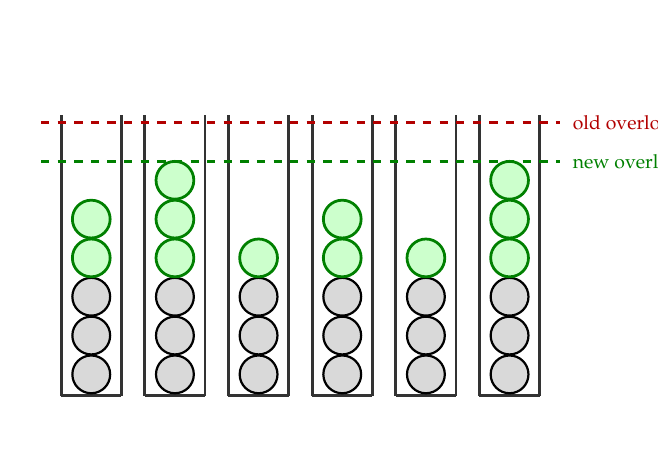
\begin{tikzpicture}[scale=0.85]
  \def\bw{0.9}
  \def\by{0}
  \def\bgap{0.35}
  \def\bs{0.48cm}
  \def\bsp{0.58}

  % Fixed bounding box (same as animation)
  \path[use as bounding box] (-0.5, -0.5) rectangle (8.5, 5.5);

  % ---- Draw 6 bins ----
  \foreach \i in {0,...,5} {
    \pgfmathsetmacro{\xx}{\i*(\bw+\bgap)}
    \draw[line width=1pt, black!80] (\xx,\by) -- (\xx,4.2);
    \draw[line width=1pt, black!80] ({\xx+\bw},\by) -- ({\xx+\bw},4.2);
    \draw[line width=1pt, black!80] (\xx,\by) -- ({\xx+\bw},\by);
  }

  % ---- Base balls (3 grey per bin) ----
  \foreach \bin in {0,...,5} {
    \foreach \j in {1,...,3} {
      \pgfmathsetmacro{\bx}{\bin*(\bw+\bgap)+0.5*\bw}
      \pgfmathsetmacro{\byy}{\by+0.32+(\j-1)*\bsp}
      \node[circle, draw, minimum size=\bs, inner sep=0pt, line width=0.8pt, fill=black!15] at (\bx,\byy) {};
    }
  }

  % ---- Green spread balls (matching overlay 4: loads 5,6,4,5,4,6) ----
  % Bin 0: +2 green (levels 4–5)
  \foreach \j in {4,5} {
    \pgfmathsetmacro{\bx}{0*(\bw+\bgap)+0.5*\bw}
    \pgfmathsetmacro{\byy}{\by+0.32+(\j-1)*\bsp}
    \node[circle, draw=green!50!black, minimum size=\bs, inner sep=0pt,
          line width=1pt, fill=green!20] at (\bx,\byy) {};
  }
  % Bin 1: +3 green (levels 4–6)
  \foreach \j in {4,5,6} {
    \pgfmathsetmacro{\bx}{1*(\bw+\bgap)+0.5*\bw}
    \pgfmathsetmacro{\byy}{\by+0.32+(\j-1)*\bsp}
    \node[circle, draw=green!50!black, minimum size=\bs, inner sep=0pt,
          line width=1pt, fill=green!20] at (\bx,\byy) {};
  }
  % Bin 2: +1 green (level 4)
  \pgfmathsetmacro{\bx}{2*(\bw+\bgap)+0.5*\bw}
  \pgfmathsetmacro{\byy}{\by+0.32+(4-1)*\bsp}
  \node[circle, draw=green!50!black, minimum size=\bs, inner sep=0pt,
        line width=1pt, fill=green!20] at (\bx,\byy) {};
  % Bin 3: +2 green (levels 4–5)
  \foreach \j in {4,5} {
    \pgfmathsetmacro{\bx}{3*(\bw+\bgap)+0.5*\bw}
    \pgfmathsetmacro{\byy}{\by+0.32+(\j-1)*\bsp}
    \node[circle, draw=green!50!black, minimum size=\bs, inner sep=0pt,
          line width=1pt, fill=green!20] at (\bx,\byy) {};
  }
  % Bin 4: +1 green (level 4)
  \pgfmathsetmacro{\bx}{4*(\bw+\bgap)+0.5*\bw}
  \pgfmathsetmacro{\byy}{\by+0.32+(4-1)*\bsp}
  \node[circle, draw=green!50!black, minimum size=\bs, inner sep=0pt,
        line width=1pt, fill=green!20] at (\bx,\byy) {};
  % Bin 5: +3 green (levels 4–6)
  \foreach \j in {4,5,6} {
    \pgfmathsetmacro{\bx}{5*(\bw+\bgap)+0.5*\bw}
    \pgfmathsetmacro{\byy}{\by+0.32+(\j-1)*\bsp}
    \node[circle, draw=green!50!black, minimum size=\bs, inner sep=0pt,
          line width=1pt, fill=green!20] at (\bx,\byy) {};
  }

  % ======== OVERLOAD LINES ========
  % Horizontal line: new overload at top of 6 balls  (y = 3.50)
  \draw[line width=1.2pt, green!50!black, dashed] (-0.3, 3.50) -- (7.45, 3.50);
  \node[right, font=\scriptsize, green!50!black] at (7.5, 3.50) {new overload};

  % Horizontal line: old overload at top of 7 balls  (y = 4.08)
  \draw[line width=1.2pt, red!70!black, dashed] (-0.3, 4.08) -- (7.45, 4.08);
  \node[right, font=\scriptsize, red!70!black] at (7.5, 4.08) {old overload};

\end{tikzpicture}
\end{center}

\vfill
1. \textbf{Slice} off the jagged surface\\
2. \textbf{Spread} balls to their second-choice bins

\end{frame}
% ===== END HIGH-WATER MARK SLIDE =====

% ===== GENERAL HISTOGRAM: Slice and Spread =====
% Initial heights (avg=3.0): 2.4, 3.6, 2.8, 3.4, 2.2, 3.8, 2.6, 3.2
% After heights  (avg=3.0): 2.9, 3.2, 3.0, 2.8, 3.1, 3.3, 2.7, 3.0
% Slice at y=2.2 (m/n - tilde-O(sqrt(m/n)))
\begin{frame}{Slice and Spread Reduces Overload}
\begin{center}
\begin{tikzpicture}[scale=0.85]
  \def\bw{0.7}
  \def\bgap{0.2}

  % Fixed bounding box
  \path[use as bounding box] (-0.5, -0.8) rectangle (9.5, 5.0);

  % Bar heights stored in macros
  % Initial: 2.4, 3.6, 2.8, 3.4, 2.2, 3.8, 2.6, 3.2
  % After:   2.9, 3.2, 3.0, 2.8, 3.1, 3.3, 2.7, 3.0
  \def\initheights{{2.4, 3.6, 2.8, 3.4, 2.2, 3.8, 2.6, 3.2}}
  \def\afterheights{{2.9, 3.2, 3.0, 2.8, 3.1, 3.3, 2.7, 3.0}}
  \def\sliceY{2.2}
  \def\meanY{3.0}

  % ======== Overlay 1: Initial state ========
  \only<1>{
    % Draw 8 grey bars
    \foreach \i in {0,...,7} {
      \pgfmathsetmacro{\xx}{\i*(\bw+\bgap)}
      \pgfmathsetmacro{\h}{\initheights[\i]}
      \fill[black!20, draw=black!50, line width=0.6pt] (\xx, 0) rectangle ({\xx+\bw}, \h);
    }

  }

  % ======== Overlays 2-6: Red tops + brace says "jaggedness" ========
  \only<2-6>{
    % Draw bars in two parts: grey below slice, red above
    \foreach \i in {0,...,7} {
      \pgfmathsetmacro{\xx}{\i*(\bw+\bgap)}
      \pgfmathsetmacro{\h}{\initheights[\i]}
      % Grey part (below slice)
      \pgfmathsetmacro{\greyTop}{min(\h, \sliceY)}
      \fill[black!20, draw=black!50, line width=0.6pt] (\xx, 0) rectangle ({\xx+\bw}, \greyTop);
      % Red part (above slice, if any)
      \pgfmathparse{\h > \sliceY ? 1 : 0}
      \ifnum\pgfmathresult=1
        \fill[red!25, draw=red!60!black, line width=0.6pt] (\xx, \sliceY) rectangle ({\xx+\bw}, \h);
      \fi
    }

    % Curly brace on the right: spans 2.2 to 3.8
    \draw[decorate, decoration={brace, amplitude=6pt, mirror}, line width=0.8pt]
          (8.4, 2.2) -- (8.4, 3.8);
    \only<2-3>{
      \node[right, font=\normalsize] at (8.65, 3.0) {jaggedness};
    }
    \only<4-6>{
      \node[right, font=\normalsize] at (8.65, 3.4) {jaggedness};
      \node[right, font=\normalsize] at (8.65, 2.5) {$\approx\Big(\dfrac{m}{n}\Big)^{1/2}$};
    }
  }

  % ======== Overlays 5-6: Slice line + scissors ========
  \only<5-6>{
    \draw[dashed, line width=1.5pt, red!70!black] (-0.3, \sliceY) -- (7.9, \sliceY);
    \node[left, red!70!black, font=\Large] at (-0.5, \sliceY) {\ding{34}};
  }

  % ======== Overlays 7-9: After spreading ========
  \only<7-9>{
    % Draw 8 bars: grey below slice, green above (the spread portion)
    \foreach \i in {0,...,7} {
      \pgfmathsetmacro{\xx}{\i*(\bw+\bgap)}
      \pgfmathsetmacro{\h}{\afterheights[\i]}
      % Grey part (below slice height)
      \pgfmathsetmacro{\greyTop}{min(\h, \sliceY)}
      \fill[black!20, draw=black!50, line width=0.6pt] (\xx, 0) rectangle ({\xx+\bw}, \greyTop);
      % Green part (above slice height, if any)
      \pgfmathparse{\h > \sliceY ? 1 : 0}
      \ifnum\pgfmathresult=1
        \fill[green!20, draw=green!50!black, line width=0.6pt] (\xx, \sliceY) rectangle ({\xx+\bw}, \h);
      \fi
    }
  }
  % Curly brace (overlays 8-9 only)
  \only<8-9>{
    \draw[decorate, decoration={brace, amplitude=6pt, mirror}, line width=0.8pt]
          (8.4, 2.7) -- (8.4, 3.3);
    \only<9>{
      \node[right, font=\normalsize] at (8.65, 3.0) {$\approx\Big(\dfrac{m}{n}\Big)^{1/4}$};
    }
  }

  % ======== Axes (always visible) ========
  % x-axis
  \draw[line width=0.8pt, black!60] (-0.3, 0) -- (7.9, 0);
  % y-axis
  \draw[line width=0.8pt, black!60] (-0.3, 0) -- (-0.3, 4.2);
  % m/n tick on y-axis
  \draw[line width=0.8pt, black!60] (-0.45, \meanY) -- (-0.3, \meanY);
  \node[left, font=\normalsize] at (-0.5, \meanY) {$\dfrac{m}{n}$};

  % Bin label centered below
  \pgfmathsetmacro{\midx}{3.5*(\bw+\bgap)+0.5*\bw}
  \node[font=\footnotesize] at (\midx, -0.4) {$n$ bins};

\end{tikzpicture}
\end{center}

\vspace{0.15cm}

\only<3-4>{
\textbf{Q:} How much is the jaggedness?
}
\only<4>{
\\[2pt]\textbf{A:} For $m \gg n$, the jaggedness is $\approx (m/n)^{1/2}$ \quad (whp in $n$)
}
\only<6-9>{
Balls sliced away: $m^{\prime} \approx n \cdot (m/n)^{1/2} = (mn)^{1/2}$
}
\only<8-9>{
\\[2pt]\textbf{Q:} What is the new jaggedness?
}
\only<9>{
\\[2pt]\textbf{A:} For $m^{\prime} \gg n$, the new jaggedness is $(m^{\prime}/n)^{1/2} = (m/n)^{1/4}$
}

\end{frame}
% ===== END GENERAL HISTOGRAM =====

\begin{frame}{Slice and Spread}
\begin{itemize}
  \item Overload: $(m/n)^{1/2} \;\to\; (m/n)^{1/4}$
  \only<2->{\item History independent? \only<3->{Yes!}}
  \only<4->{\item Recourse: \only<5->{$1^{*}$}}
\end{itemize}

% ---- Overlay 6-7: recourse picture (blue x inserted at level 3, pushes grey up) ----
\only<6->{\vspace{0.2cm}\hspace{0.5cm}\textbf{Example}\vspace{-0.2cm}}
\only<6-7>{
\noindent\hspace*{-0.5\dimexpr\paperwidth-\textwidth\relax}%
\makebox[\paperwidth][c]{%
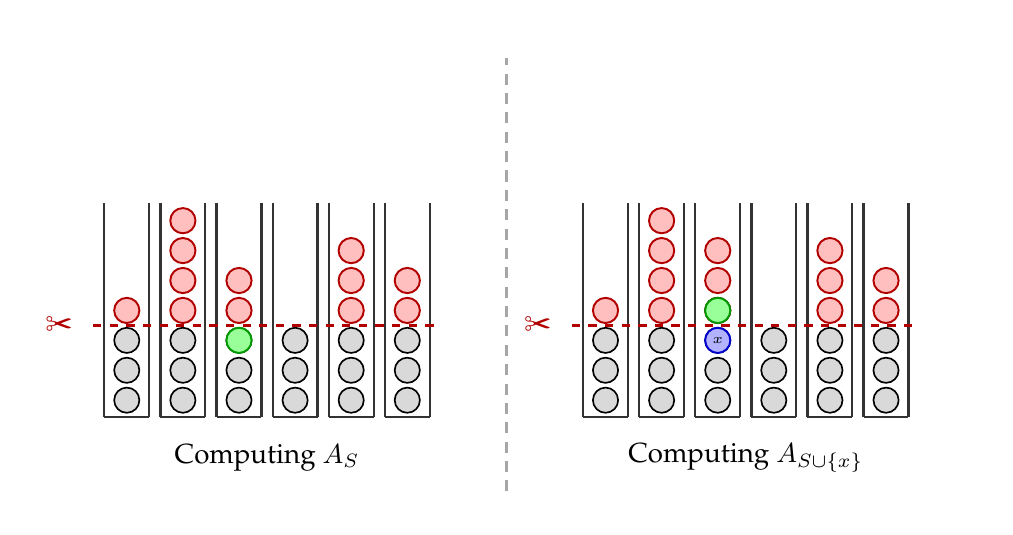
\begin{tikzpicture}[x=1cm,y=1cm,scale=0.95]
  \path[use as bounding box] (-6.4,-3.2) rectangle (6.4,3.2);
  \draw[dash pattern=on 4pt off 3pt, line width=0.8pt, black!35] (0,-3.0) -- (0,2.8);
  \def\bw{0.6}\def\bgap{0.15}\def\bs{0.32cm}\def\bsp{0.40}\def\boffset{0.22}\def\biny{-2.0}
  \pgfmathsetmacro{\wallTop}{\biny + 2.85}
  \pgfmathsetmacro{\sliceY}{\biny + \boffset + 2.5*\bsp}
  \foreach \wx in {-5.375, 1.025} {
    \foreach \i in {0,...,5} {
      \pgfmathsetmacro{\xx}{\wx + \i*(\bw+\bgap)}
      \draw[line width=0.8pt, black!80] (\xx,\biny) -- (\xx,\wallTop);
      \draw[line width=0.8pt, black!80] ({\xx+\bw},\biny) -- ({\xx+\bw},\wallTop);
      \draw[line width=0.8pt, black!80] (\xx,\biny) -- ({\xx+\bw},\biny);
    }
    \foreach \bin in {0,...,5} {
      \foreach \j in {1,...,3} {
        \pgfmathsetmacro{\bx}{\wx + \bin*(\bw+\bgap) + 0.5*\bw}
        \pgfmathsetmacro{\byy}{\biny + \boffset + (\j-1)*\bsp}
        \node[circle, draw, minimum size=\bs, inner sep=0pt, line width=0.6pt, fill=black!15] at (\bx,\byy) {};
      }
    }
    \pgfmathsetmacro{\sliceLeft}{\wx - 0.15}
    \pgfmathsetmacro{\sliceRight}{\wx + 5*(\bw+\bgap) + \bw + 0.1}
    \draw[dashed, line width=1.2pt, red!70!black] (\sliceLeft,\sliceY) -- (\sliceRight,\sliceY);
    \pgfmathsetmacro{\scissX}{\wx - 0.3}
    \node[left, red!70!black, font=\normalsize] at (\scissX,\sliceY) {\ding{34}};
    % Red balls above threshold
    \pgfmathsetmacro{\bx}{\wx + 0*(\bw+\bgap) + 0.5*\bw}
    \pgfmathsetmacro{\byy}{\biny + \boffset + 3*\bsp}
    \node[circle, draw=red!70!black, minimum size=\bs, inner sep=0pt, line width=0.7pt, fill=red!25] at (\bx,\byy) {};
    \foreach \j in {4,...,7} {
      \pgfmathsetmacro{\bx}{\wx + 1*(\bw+\bgap) + 0.5*\bw}
      \pgfmathsetmacro{\byy}{\biny + \boffset + (\j-1)*\bsp}
      \node[circle, draw=red!70!black, minimum size=\bs, inner sep=0pt, line width=0.7pt, fill=red!25] at (\bx,\byy) {};
    }
    \foreach \j in {4,5} {
      \pgfmathsetmacro{\bx}{\wx + 2*(\bw+\bgap) + 0.5*\bw}
      \pgfmathsetmacro{\byy}{\biny + \boffset + (\j-1)*\bsp}
      \node[circle, draw=red!70!black, minimum size=\bs, inner sep=0pt, line width=0.7pt, fill=red!25] at (\bx,\byy) {};
    }
    \foreach \j in {4,...,6} {
      \pgfmathsetmacro{\bx}{\wx + 4*(\bw+\bgap) + 0.5*\bw}
      \pgfmathsetmacro{\byy}{\biny + \boffset + (\j-1)*\bsp}
      \node[circle, draw=red!70!black, minimum size=\bs, inner sep=0pt, line width=0.7pt, fill=red!25] at (\bx,\byy) {};
    }
    \foreach \j in {4,5} {
      \pgfmathsetmacro{\bx}{\wx + 5*(\bw+\bgap) + 0.5*\bw}
      \pgfmathsetmacro{\byy}{\biny + \boffset + (\j-1)*\bsp}
      \node[circle, draw=red!70!black, minimum size=\bs, inner sep=0pt, line width=0.7pt, fill=red!25] at (\bx,\byy) {};
    }
  }
  % Right-world bin 2: blue x at level 3, grey pushed to level 4, red pushed to level 6
  \pgfmathsetmacro{\bx}{1.025 + 2*(\bw+\bgap) + 0.5*\bw}
  \pgfmathsetmacro{\byy}{\biny + \boffset + 2*\bsp}
  \node[circle, draw=blue!80!black, minimum size=\bs, inner sep=0pt, line width=0.7pt, fill=blue!30, font=\tiny] at (\bx,\byy) {$x$};
  \pgfmathsetmacro{\byy}{\biny + \boffset + 3*\bsp}
  \node[circle, draw, minimum size=\bs, inner sep=0pt, line width=0.6pt, fill=black!15] at (\bx,\byy) {};
  \pgfmathsetmacro{\byy}{\biny + \boffset + 5*\bsp}
  \node[circle, draw=red!70!black, minimum size=\bs, inner sep=0pt, line width=0.7pt, fill=red!25] at (\bx,\byy) {};
  % Labels
  \node[font=\normalsize] at (-3.2, -2.55) {Computing $A_S$};
  \node[font=\normalsize] at (3.2, -2.55) {Computing $A_{S \cup \{x\}}$};
  % Overlay 7: highlight matching balls in orange
  \only<7>{
    % Left picture, bin 2, top grey ball (level 3) turns orange
    \pgfmathsetmacro{\bxLO}{-5.375 + 2*(\bw+\bgap) + 0.5*\bw}
    \pgfmathsetmacro{\byyLO}{\biny + \boffset + 2*\bsp}
    \node[circle, draw=green!60!black, minimum size=\bs, inner sep=0pt, line width=0.7pt, fill=green!40] at (\bxLO,\byyLO) {};
    % Right picture, bin 2, grey ball above blue x (level 4) turns green
    \pgfmathsetmacro{\bxRO}{1.025 + 2*(\bw+\bgap) + 0.5*\bw}
    \pgfmathsetmacro{\byyRO}{\biny + \boffset + 3*\bsp}
    \node[circle, draw=green!60!black, minimum size=\bs, inner sep=0pt, line width=0.7pt, fill=green!40] at (\bxRO,\byyRO) {};
  }
\end{tikzpicture}
}%
}
\end{frame}

\begin{frame}{Repeatedly Slicing and Spreading}
\begin{center}
\begin{tikzpicture}[scale=0.85]
  \path[use as bounding box] (-0.5, -1.2) rectangle (12.5, 3.8);

  % --- Helper: draw a small histogram at (xoff, 0) with given bar heights ---
  % Round 0: tall jagged bars
  \foreach \i/\h in {0/2.4, 1/3.2, 2/2.6, 3/3.4, 4/2.2, 5/3.6} {
    \pgfmathsetmacro{\xx}{0 + \i*0.35}
    \fill[black!25] (\xx, 0) rectangle ({\xx+0.3}, \h);
    \draw[line width=0.4pt, black!50] (\xx, 0) rectangle ({\xx+0.3}, \h);
  }
  \draw[line width=0.6pt, black!60] (0,0) -- (2.05,0);
  \node[font=\scriptsize, below] at (1.0, -0.1) {Round $1$};
  \node[font=\scriptsize, above, text=black!70] at (1.0, 3.5) {$\tilde{O}\Big(\dfrac{m}{n}\Big)^{1/2}$};

  % Arrow
  \draw[->, line width=1pt, black!60] (2.3, 1.5) -- (3.0, 1.5);

  % Round 1: less jagged
  \foreach \i/\h in {0/2.7, 1/3.0, 2/2.8, 3/3.1, 4/2.6, 5/3.2} {
    \pgfmathsetmacro{\xx}{3.3 + \i*0.35}
    \fill[black!25] (\xx, 0) rectangle ({\xx+0.3}, \h);
    \draw[line width=0.4pt, black!50] (\xx, 0) rectangle ({\xx+0.3}, \h);
  }
  \draw[line width=0.6pt, black!60] (3.3,0) -- (5.35,0);
  \node[font=\scriptsize, below] at (4.3, -0.1) {Round $2$};
  \node[font=\scriptsize, above, text=black!70] at (4.3, 3.5) {$\tilde{O}\Big(\dfrac{m}{n}\Big)^{1/4}$};

  % Arrow
  \draw[->, line width=1pt, black!60] (5.6, 1.5) -- (6.3, 1.5);

  % Round 2: even flatter
  \foreach \i/\h in {0/2.85, 1/2.95, 2/2.88, 3/3.02, 4/2.82, 5/3.05} {
    \pgfmathsetmacro{\xx}{6.6 + \i*0.35}
    \fill[black!25] (\xx, 0) rectangle ({\xx+0.3}, \h);
    \draw[line width=0.4pt, black!50] (\xx, 0) rectangle ({\xx+0.3}, \h);
  }
  \draw[line width=0.6pt, black!60] (6.6,0) -- (8.65,0);
  \node[font=\scriptsize, below] at (7.6, -0.1) {Round $3$};
  \node[font=\scriptsize, above, text=black!70] at (7.6, 3.5) {$\tilde{O}\Big(\dfrac{m}{n}\Big)^{1/8}$};

  % Dots
  \node[font=\large] at (9.3, 1.5) {$\cdots$};

\end{tikzpicture}
\end{center}
\pause
\only<2>{
After $O(\log \log (m/n))$ rounds\ldots
\begin{itemize}
\item Overload $= O(1)$?
\item Recourse $= O(\log \log (m/n))$?
\end{itemize}
}
% \only<3>{
% \sout{After $O(\log \log (m/n))$ rounds\ldots}
% \begin{itemize}
% \item \sout{Overload $= O(1)$?}
% \item \sout{Recourse $= O(\log \log (m/n))$?}
% \end{itemize}
% }

\end{frame}

\begin{frame}{Algorithmic Question}

\begin{center}
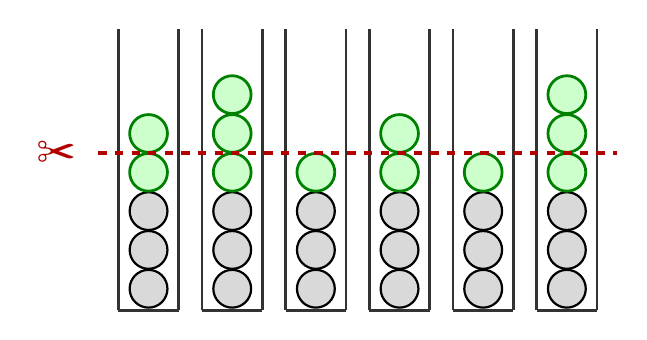
\begin{tikzpicture}[scale=0.85]
  \def\bw{0.9}
  \def\by{0}
  \def\bgap{0.35}
  \def\bs{0.48cm}
  \def\bsp{0.58}

  % Draw 6 bins
  \foreach \i in {0,...,5} {
    \pgfmathsetmacro{\xx}{\i*(\bw+\bgap)}
    \draw[line width=1pt, black!80] (\xx,\by) -- (\xx,4.2);
    \draw[line width=1pt, black!80] ({\xx+\bw},\by) -- ({\xx+\bw},4.2);
    \draw[line width=1pt, black!80] (\xx,\by) -- ({\xx+\bw},\by);
  }

  % Grey balls (3 per bin)
  \foreach \bin in {0,...,5} {
    \foreach \j in {1,...,3} {
      \pgfmathsetmacro{\bx}{\bin*(\bw+\bgap)+0.5*\bw}
      \pgfmathsetmacro{\byy}{\by+0.32+(\j-1)*\bsp}
      \node[circle, draw, minimum size=\bs, inner sep=0pt, line width=0.8pt, fill=black!15] at (\bx,\byy) {};
    }
  }

  % Green balls above threshold (post-spread)
  % Bin 0: +2 green (levels 4-5)
  \foreach \j in {4,5} {
    \pgfmathsetmacro{\bx}{0*(\bw+\bgap)+0.5*\bw}
    \pgfmathsetmacro{\byy}{\by+0.32+(\j-1)*\bsp}
    \node[circle, draw=green!50!black, minimum size=\bs, inner sep=0pt, line width=1pt, fill=green!20] at (\bx,\byy) {};
  }
  % Bin 1: +3 green (levels 4-6)
  \foreach \j in {4,5,6} {
    \pgfmathsetmacro{\bx}{1*(\bw+\bgap)+0.5*\bw}
    \pgfmathsetmacro{\byy}{\by+0.32+(\j-1)*\bsp}
    \node[circle, draw=green!50!black, minimum size=\bs, inner sep=0pt, line width=1pt, fill=green!20] at (\bx,\byy) {};
  }
  % Bin 2: +1 green (level 4)
  \pgfmathsetmacro{\bx}{2*(\bw+\bgap)+0.5*\bw}
  \pgfmathsetmacro{\byy}{\by+0.32+(4-1)*\bsp}
  \node[circle, draw=green!50!black, minimum size=\bs, inner sep=0pt, line width=1pt, fill=green!20] at (\bx,\byy) {};
  % Bin 3: +2 green (levels 4-5)
  \foreach \j in {4,5} {
    \pgfmathsetmacro{\bx}{3*(\bw+\bgap)+0.5*\bw}
    \pgfmathsetmacro{\byy}{\by+0.32+(\j-1)*\bsp}
    \node[circle, draw=green!50!black, minimum size=\bs, inner sep=0pt, line width=1pt, fill=green!20] at (\bx,\byy) {};
  }
  % Bin 4: +1 green (level 4)
  \pgfmathsetmacro{\bx}{4*(\bw+\bgap)+0.5*\bw}
  \pgfmathsetmacro{\byy}{\by+0.32+(4-1)*\bsp}
  \node[circle, draw=green!50!black, minimum size=\bs, inner sep=0pt, line width=1pt, fill=green!20] at (\bx,\byy) {};
  % Bin 5: +3 green (levels 4-6)
  \foreach \j in {4,5,6} {
    \pgfmathsetmacro{\bx}{5*(\bw+\bgap)+0.5*\bw}
    \pgfmathsetmacro{\byy}{\by+0.32+(\j-1)*\bsp}
    \node[circle, draw=green!50!black, minimum size=\bs, inner sep=0pt, line width=1pt, fill=green!20] at (\bx,\byy) {};
  }

  % Dashed slice line at height of 4 balls (between levels 4 and 5)
  \pgfmathsetmacro{\sliceY}{\by+0.32+3*\bsp+0.5*\bsp}
  \draw[dashed, line width=1.5pt, red!70!black] (-0.3,\sliceY) -- (7.45,\sliceY);
  \node[left, red!70!black, font=\Large] at (-0.5,\sliceY) {\ding{34}};

\end{tikzpicture}
\end{center}

\begin{center}
\textbf{Question:} Which balls do we slice in round $k$?
\end{center}

\pause

\hspace*{-0.5cm}\parbox{\dimexpr\textwidth+0.5cm}{%
\begin{itemize}
  \item \textbf{Option 1:} Scrape off the top \only<3->{\hfill {\color{red}\ding{55}} \small Reuses stale randomness \normalsize}
  \only<4->{\item \textbf{Option 2:} Priority queue per bin \only<5->{\hfill {\color{red}\ding{55}} \small Exploding recourse \normalsize}}
  \only<6->{\item \textbf{Our approach:} Assign every ball a random \textbf{round number}, only choose from the balls with round number $k$}
\end{itemize}
}

\end{frame}

\begin{frame}{Challenge $1$: Slicing Failures}

\begin{center}
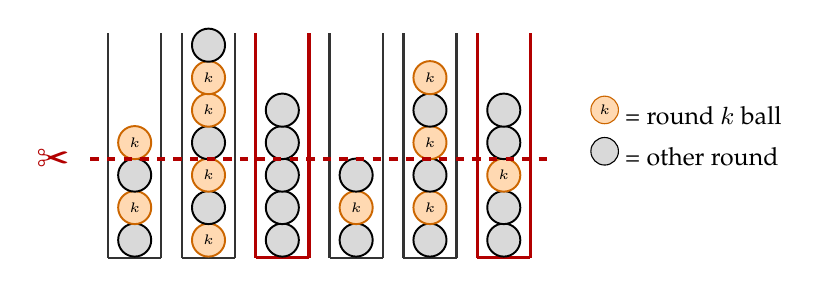
\begin{tikzpicture}[scale=0.75]
  \def\bw{0.9}
  \def\by{0}
  \def\bgap{0.35}
  \def\bs{0.42cm}
  \def\bsp{0.55}

  % Draw 6 bins (bins 2 and 5 in red for failure)
  \foreach \i in {0,1,3,4} {
    \pgfmathsetmacro{\xx}{\i*(\bw+\bgap)}
    \draw[line width=0.8pt, black!80] (\xx,\by) -- (\xx,3.8);
    \draw[line width=0.8pt, black!80] ({\xx+\bw},\by) -- ({\xx+\bw},3.8);
    \draw[line width=0.8pt, black!80] (\xx,\by) -- ({\xx+\bw},\by);
  }
  \foreach \i in {2,5} {
    \pgfmathsetmacro{\xx}{\i*(\bw+\bgap)}
    \draw[line width=1.2pt, red!70!black] (\xx,\by) -- (\xx,3.8);
    \draw[line width=1.2pt, red!70!black] ({\xx+\bw},\by) -- ({\xx+\bw},3.8);
    \draw[line width=1.2pt, red!70!black] (\xx,\by) -- ({\xx+\bw},\by);
  }

  % Ball styles
  \tikzset{
    gb/.style={circle, draw, minimum size=\bs, inner sep=0pt, line width=0.7pt, fill=black!15},
    kb/.style={circle, draw=orange!80!black, minimum size=\bs, inner sep=0pt, line width=0.7pt, fill=orange!30, font=\tiny}
  }

  % Bin 0: 4 balls, 2 orange — grey, orange, grey, orange
  \pgfmathsetmacro{\bx}{0*(\bw+\bgap)+0.5*\bw}
  \node[gb] at (\bx,{\by+0.30+0*\bsp}) {};
  \node[kb] at (\bx,{\by+0.30+1*\bsp}) {$k$};
  \node[gb] at (\bx,{\by+0.30+2*\bsp}) {};
  \node[kb] at (\bx,{\by+0.30+3*\bsp}) {$k$};

  % Bin 1: 7 balls, 4 orange — orange, grey, orange, grey, orange, orange, grey
  \pgfmathsetmacro{\bx}{1*(\bw+\bgap)+0.5*\bw}
  \node[kb] at (\bx,{\by+0.30+0*\bsp}) {$k$};
  \node[gb] at (\bx,{\by+0.30+1*\bsp}) {};
  \node[kb] at (\bx,{\by+0.30+2*\bsp}) {$k$};
  \node[gb] at (\bx,{\by+0.30+3*\bsp}) {};
  \node[kb] at (\bx,{\by+0.30+4*\bsp}) {$k$};
  \node[kb] at (\bx,{\by+0.30+5*\bsp}) {$k$};
  \node[gb] at (\bx,{\by+0.30+6*\bsp}) {};

  % Bin 2: 5 balls, 0 orange — all grey
  \pgfmathsetmacro{\bx}{2*(\bw+\bgap)+0.5*\bw}
  \foreach \j in {0,...,4} {
    \node[gb] at (\bx,{\by+0.30+\j*\bsp}) {};
  }

  % Bin 3: 3 balls, 1 orange — grey, orange, grey
  \pgfmathsetmacro{\bx}{3*(\bw+\bgap)+0.5*\bw}
  \node[gb] at (\bx,{\by+0.30+0*\bsp}) {};
  \node[kb] at (\bx,{\by+0.30+1*\bsp}) {$k$};
  \node[gb] at (\bx,{\by+0.30+2*\bsp}) {};

  % Bin 4: 6 balls, 3 orange — grey, orange, grey, orange, grey, orange
  \pgfmathsetmacro{\bx}{4*(\bw+\bgap)+0.5*\bw}
  \node[gb] at (\bx,{\by+0.30+0*\bsp}) {};
  \node[kb] at (\bx,{\by+0.30+1*\bsp}) {$k$};
  \node[gb] at (\bx,{\by+0.30+2*\bsp}) {};
  \node[kb] at (\bx,{\by+0.30+3*\bsp}) {$k$};
  \node[gb] at (\bx,{\by+0.30+4*\bsp}) {};
  \node[kb] at (\bx,{\by+0.30+5*\bsp}) {$k$};

  % Bin 5: 5 balls, 1 orange — grey, grey, orange, grey, grey
  \pgfmathsetmacro{\bx}{5*(\bw+\bgap)+0.5*\bw}
  \node[gb] at (\bx,{\by+0.30+0*\bsp}) {};
  \node[gb] at (\bx,{\by+0.30+1*\bsp}) {};
  \node[kb] at (\bx,{\by+0.30+2*\bsp}) {$k$};
  \node[gb] at (\bx,{\by+0.30+3*\bsp}) {};
  \node[gb] at (\bx,{\by+0.30+4*\bsp}) {};

  % Slice line
  \pgfmathsetmacro{\sliceY}{\by+0.30+2.5*\bsp}
  \draw[dashed, line width=1.2pt, red!70!black] (-0.3,\sliceY) -- (7.45,\sliceY);
  \node[left, red!70!black, font=\large] at (-0.5,\sliceY) {\ding{34}};

  % Legend
  \node[right, font=\small] at (8.0, 2.5) {\tikz\node[circle, draw=orange!80!black, minimum size=0.35cm, inner sep=0pt, fill=orange!30, font=\tiny]{$k$}; = round $k$ ball};
  \node[right, font=\small] at (8.0, 1.8) {\tikz\node[circle, draw, minimum size=0.35cm, inner sep=0pt, fill=black!15]{}; = other round};

\end{tikzpicture}
\end{center}

\pause

\textbf{Challenge:} Some bins may not have enough round-$k$ balls to support slicing.

\pause

\textbf{Result:} We can't slice evenly --- the jaggedness remains in those bins.

\end{frame}

\begin{frame}{Challenge $2$: Spreading Failures}

\begin{center}
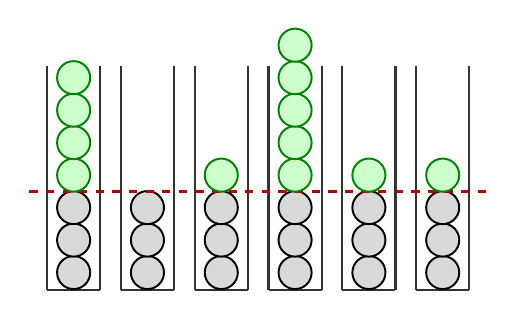
\begin{tikzpicture}[scale=0.75]
  \def\bw{0.9}
  \def\by{0}
  \def\bgap{0.35}
  \def\bs{0.42cm}
  \def\bsp{0.55}

  % Draw 6 bins
  \foreach \i in {0,...,5} {
    \pgfmathsetmacro{\xx}{\i*(\bw+\bgap)}
    \draw[line width=0.8pt, black!80] (\xx,\by) -- (\xx,3.8);
    \draw[line width=0.8pt, black!80] ({\xx+\bw},\by) -- ({\xx+\bw},3.8);
    \draw[line width=0.8pt, black!80] (\xx,\by) -- ({\xx+\bw},\by);
  }

  % Grey balls below slice (3 per bin)
  \foreach \bin in {0,...,5} {
    \foreach \j in {1,...,3} {
      \pgfmathsetmacro{\bx}{\bin*(\bw+\bgap)+0.5*\bw}
      \pgfmathsetmacro{\byy}{\by+0.30+(\j-1)*\bsp}
      \node[circle, draw, minimum size=\bs, inner sep=0pt, line width=0.7pt, fill=black!15] at (\bx,\byy) {};
    }
  }

  % Slice line
  \pgfmathsetmacro{\sliceY}{\by+0.30+2.5*\bsp}
  \draw[dashed, line width=1.2pt, red!70!black] (-0.3,\sliceY) -- (7.45,\sliceY);

  % Green balls after spreading — very uneven distribution!
  % Bin 0: +4 green (levels 4-7) — way too many
  \foreach \j in {4,...,7} {
    \pgfmathsetmacro{\bx}{0*(\bw+\bgap)+0.5*\bw}
    \pgfmathsetmacro{\byy}{\by+0.30+(\j-1)*\bsp}
    \node[circle, draw=green!50!black, minimum size=\bs, inner sep=0pt, line width=0.7pt, fill=green!20] at (\bx,\byy) {};
  }
  % Bin 1: +0 green — got nothing
  % Bin 2: +1 green (level 4)
  \pgfmathsetmacro{\bx}{2*(\bw+\bgap)+0.5*\bw}
  \pgfmathsetmacro{\byy}{\by+0.30+3*\bsp}
  \node[circle, draw=green!50!black, minimum size=\bs, inner sep=0pt, line width=0.7pt, fill=green!20] at (\bx,\byy) {};
  % Bin 3: +5 green (levels 4-8) — way too many
  \foreach \j in {4,...,8} {
    \pgfmathsetmacro{\bx}{3*(\bw+\bgap)+0.5*\bw}
    \pgfmathsetmacro{\byy}{\by+0.30+(\j-1)*\bsp}
    \node[circle, draw=green!50!black, minimum size=\bs, inner sep=0pt, line width=0.7pt, fill=green!20] at (\bx,\byy) {};
  }
  % Bin 4: +1 green (level 4)
  \pgfmathsetmacro{\bx}{4*(\bw+\bgap)+0.5*\bw}
  \pgfmathsetmacro{\byy}{\by+0.30+3*\bsp}
  \node[circle, draw=green!50!black, minimum size=\bs, inner sep=0pt, line width=0.7pt, fill=green!20] at (\bx,\byy) {};
  % Bin 5: +1 green (level 4)
  \pgfmathsetmacro{\bx}{5*(\bw+\bgap)+0.5*\bw}
  \pgfmathsetmacro{\byy}{\by+0.30+3*\bsp}
  \node[circle, draw=green!50!black, minimum size=\bs, inner sep=0pt, line width=0.7pt, fill=green!20] at (\bx,\byy) {};


\end{tikzpicture}
\end{center}

\pause

\textbf{Challenge:} The spreading step may distribute balls unevenly --- creating new jaggedness.

\pause

\textbf{Dilemma:}
\begin{itemize}
  \item Slice \textbf{more} balls $\implies$ overload may not decrease
  \item Slice \textbf{fewer} balls $\implies$ jaggedness may not decrease
\end{itemize}

\end{frame}

\begin{frame}{Repeatedly Slicing and Spreading}
  \begin{center}
  \begin{tikzpicture}[scale=0.85]
    \path[use as bounding box] (-0.5, -1.2) rectangle (12.5, 3.8);
  
    % --- Helper: draw a small histogram at (xoff, 0) with given bar heights ---
    % Round 0: tall jagged bars
    \foreach \i/\h in {0/2.4, 1/3.2, 2/2.6, 3/3.4, 4/2.2, 5/3.6} {
      \pgfmathsetmacro{\xx}{0 + \i*0.35}
      \fill[black!25] (\xx, 0) rectangle ({\xx+0.3}, \h);
      \draw[line width=0.4pt, black!50] (\xx, 0) rectangle ({\xx+0.3}, \h);
    }
    \draw[line width=0.6pt, black!60] (0,0) -- (2.05,0);
    \node[font=\scriptsize, below] at (1.0, -0.1) {Round $1$};
    \node[font=\scriptsize, above, text=black!70] at (1.0, 3.5) {$\tilde{O}\Big(\dfrac{m}{n}\Big)^{1/2}$};
  
    % Arrow
    \draw[->, line width=1pt, black!60] (2.3, 1.5) -- (3.0, 1.5);
  
    % Round 1: less jagged
    \foreach \i/\h in {0/2.7, 1/3.0, 2/2.8, 3/3.1, 4/2.6, 5/3.2} {
      \pgfmathsetmacro{\xx}{3.3 + \i*0.35}
      \fill[black!25] (\xx, 0) rectangle ({\xx+0.3}, \h);
      \draw[line width=0.4pt, black!50] (\xx, 0) rectangle ({\xx+0.3}, \h);
    }
    \draw[line width=0.6pt, black!60] (3.3,0) -- (5.35,0);
    \node[font=\scriptsize, below] at (4.3, -0.1) {Round $2$};
    \node[font=\scriptsize, above, text=black!70] at (4.3, 3.5) {$\tilde{O}\Big(\dfrac{m}{n}\Big)^{1/4}$};
  
    % Arrow
    \draw[->, line width=1pt, black!60] (5.6, 1.5) -- (6.3, 1.5);
  
    % Round 2: even flatter
    \foreach \i/\h in {0/2.85, 1/2.95, 2/2.88, 3/3.02, 4/2.82, 5/3.05} {
      \pgfmathsetmacro{\xx}{6.6 + \i*0.35}
      \fill[black!25] (\xx, 0) rectangle ({\xx+0.3}, \h);
      \draw[line width=0.4pt, black!50] (\xx, 0) rectangle ({\xx+0.3}, \h);
    }
    \draw[line width=0.6pt, black!60] (6.6,0) -- (8.65,0);
    \node[font=\scriptsize, below] at (7.6, -0.1) {Round $3$};
    \node[font=\scriptsize, above, text=black!70] at (7.6, 3.5) {$\tilde{O}\Big(\dfrac{m}{n}\Big)^{1/8}$};
  
    % Dots
    \node[font=\large] at (9.3, 1.5) {$\cdots$};
  
  \end{tikzpicture}
  \end{center}
  After $O(\log \log (m/n))$ rounds\ldots
  \begin{itemize}
    \item \sout{Overload $= O(1)$} {\color{blue} Cumulative overload $= O(n)$}
    \item Recourse $= O(\log \log (m/n))$
  \end{itemize}
  
  
  \end{frame}


\begin{frame}{Full Algorithm}


  \vspace{0.3cm}
  
  \begin{center}
  \begin{tikzpicture}[scale=1.0]
    % Timeline bar
    \def\totalW{9}
    \def\prefixW{5.5}
    \def\barH{0.8}
  
    \def\nGadgets{3}
    \pgfmathsetmacro{\gadgetW}{\prefixW/\nGadgets}
  
    % Prefix: Slice and Spread (always visible)
    \fill[blue!20] (0,0) rectangle (\prefixW,\barH);
    \draw[line width=1pt, blue!60!black] (0,0) rectangle (\prefixW,\barH);
  
    % Suffix: Patchwork (always visible)
    \fill[orange!20] (\prefixW,0) rectangle (\totalW,\barH);
    \draw[line width=1pt, orange!70!black] (\prefixW,0) rectangle (\totalW,\barH);
  
    % Labels above regions (always visible)
    \node[above, font=\normalsize] at (0.5*\prefixW, \barH+0.1) {\textbf{Slice and Spread}};
    \node[above, font=\normalsize] at ({0.5*(\prefixW+\totalW)}, \barH+0.1) {\textbf{Patch}};
  
    % Subdivided into rounds (always visible)
    \foreach \g in {1,...,2} {
      \pgfmathsetmacro{\gx}{\g*\gadgetW}
      \draw[line width=0.7pt, blue!60!black] (\gx,0) -- (\gx,\barH);
    }
    \node[font=\small] at ({0.5*\gadgetW}, 0.5*\barH) {$1$};
    \node[font=\small] at ({1.5*\gadgetW}, 0.5*\barH) {$2$};
    \node[font=\small] at ({2.5*\gadgetW}, 0.5*\barH) {$\cdots$};
  
    % Labels at left and right edges (always visible, fixed position)
    \node[font=\small, left] at (-0.1, 0.5*\barH) {start};
    \node[font=\small, right] at ({\totalW+0.1}, 0.5*\barH) {finish};

    % Arrow from below pointing up at end of blue region
    \only<1->{
      \node[below, font=\small, text width=3.8cm, align=center] (here) at (\prefixW, -1.8)
        {\textbf{We are here:}\\[2pt]
         \begin{itemize}\setlength{\itemsep}{0pt}\setlength{\parskip}{0pt}
           \item Cumulative overload $O(n)$
           \item Recourse $O(\log \log (m/n))$
         \end{itemize}};
      \draw[->, thick, blue!60!black] (here.north) -- (\prefixW, -0.15);
    }

    % Arrow from below pointing up at end of orange region
    \only<2->{
      \node[below, font=\small, text width=3.5cm, align=center] (goal) at (\totalW, -1.8)
        {\textbf{Final:}\\[2pt]
         \begin{itemize}\setlength{\itemsep}{0pt}\setlength{\parskip}{0pt}
           \item Overload $O(1)$
           \item Recourse $O(\log \log (m/n))$
         \end{itemize}};
      \draw[->, thick, orange!70!black] (goal.north) -- (\totalW, -0.15);
    }
  
  \end{tikzpicture}
  \end{center}

\end{frame}

\begin{frame}{Past Work (Not History Independent)} 

  % \textbf{Past work on insertion-only case: }
  % {\color{gray} [Azar, Broder, Karlin and Upfal '94]
  % [Berenbrink, Czumaj, Steger, and V{\"o}cking '00][Dietzfelbinger and Weidling '07] 
  % [Frieze and Petti '18] $\ldots$} \pause 
  
  \vspace{2mm}
  \begin{center}
  \renewcommand{\arraystretch}{1.3}
  \begin{tabular}{@{}cccc@{}}
  \toprule
  \textbf{Overload} & \textbf{Recourse} & \textbf{Reference} & \textbf{Caveats} \\
  \midrule
  $O(\log \log n)$ & $0$ & {\scriptsize [ABKU '94] [BCSV '00]} & {\scriptsize insertion-only} \\
  $O(1)$ & $O(\log (m/n))$ & {\scriptsize [Dietzfelbinger, Weidling '07]} & {\scriptsize insertion-only} \\
  $\tilde{O}(\sqrt{m/n})$ & $O(1)$ & {\scriptsize [Frieze, Petti '18]} & {\scriptsize insertion-only} \\
  $O(\log (m/n))$ & $0$ & {\scriptsize [Bansal, Kuszmaul '22]} & {\scriptsize no reinsertions} \\
  $O(1)$ & $O(m/n)$ & {\scriptsize [Dietzfelbinger, Weidling '07]} &  \\
  \bottomrule
  \color{blue} $O(1)$ & \color{blue} $O(\log \log (m/n))$ & \color{blue} {\scriptsize [This Paper]} & \\ 
  \bottomrule
  \end{tabular}
  \end{center}

  
  % But the fully dynamic case has remained largely open.
  
  % {\color{gray} [V{\"o}cking '99] [Dietzfelbinger and Weidling '07] [Bender, Conway, Farach-Colton, Kuszmaul, Tagliavini '21] [Bansal, Kuszmaul '22] $\ldots$} \pause
  
   \vspace{.2 cm}
  
   \color{blue}
  
  Privacy can be leveraged as an \emph{algorithmic tool} to outperform non-private algorithms!
  
  \end{frame}

\begin{frame}[plain]
  \vspace{5mm}
  \begin{center}
    {\LARGE \textbf{History-Independent Load Balancing}}
  \end{center}
  
  \vspace{6mm}
  
  \begin{center}
  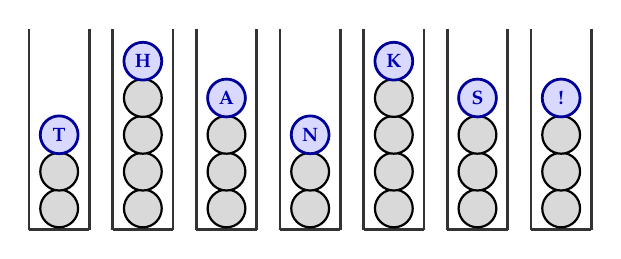
\begin{tikzpicture}[scale=0.85]
    % Exact same dimensions as Two-Choice Load Balancing slide
    \def\bw{0.9}
    \def\bh{3.0}
    \def\by{0}
    \def\bgap{0.35}
    \def\bs{0.48cm}
    \def\bsp{0.55}
    
    % Draw 7 rectangular bins
    \foreach \i in {0,...,6} {
      \pgfmathsetmacro{\xx}{\i*(\bw+\bgap)}
      \draw[line width=1pt, black!80] (\xx,\by) -- (\xx,\bh);
      \draw[line width=1pt, black!80] ({\xx+\bw},\by) -- ({\xx+\bw},\bh);
      \draw[line width=1pt, black!80] (\xx,\by) -- ({\xx+\bw},\by);
    }
    
    % Bin 0: 3 balls (top ball = T)
    \foreach \j in {1,2} {
      \pgfmathsetmacro{\bx}{0*(\bw+\bgap)+0.5*\bw}
      \pgfmathsetmacro{\byy}{\by+0.32+(\j-1)*\bsp}
      \node[circle, draw, minimum size=\bs, inner sep=0pt, line width=0.8pt, fill=black!15] at (\bx,\byy) {};
    }
    \pgfmathsetmacro{\bx}{0*(\bw+\bgap)+0.5*\bw}
    \pgfmathsetmacro{\byy}{\by+0.32+(3-1)*\bsp}
    \node[circle, draw=blue!60!black, minimum size=\bs, inner sep=0pt, line width=1pt, fill=blue!15, text=blue!70!black] at (\bx,\byy) {\scriptsize\textbf{T}};
    
    % Bin 1: 5 balls (top ball = H)
    \foreach \j in {1,2,3,4} {
      \pgfmathsetmacro{\bx}{1*(\bw+\bgap)+0.5*\bw}
      \pgfmathsetmacro{\byy}{\by+0.32+(\j-1)*\bsp}
      \node[circle, draw, minimum size=\bs, inner sep=0pt, line width=0.8pt, fill=black!15] at (\bx,\byy) {};
    }
    \pgfmathsetmacro{\bx}{1*(\bw+\bgap)+0.5*\bw}
    \pgfmathsetmacro{\byy}{\by+0.32+(5-1)*\bsp}
    \node[circle, draw=blue!60!black, minimum size=\bs, inner sep=0pt, line width=1pt, fill=blue!15, text=blue!70!black] at (\bx,\byy) {\scriptsize\textbf{H}};
    
    % Bin 2: 4 balls (top ball = A)
    \foreach \j in {1,2,3} {
      \pgfmathsetmacro{\bx}{2*(\bw+\bgap)+0.5*\bw}
      \pgfmathsetmacro{\byy}{\by+0.32+(\j-1)*\bsp}
      \node[circle, draw, minimum size=\bs, inner sep=0pt, line width=0.8pt, fill=black!15] at (\bx,\byy) {};
    }
    \pgfmathsetmacro{\bx}{2*(\bw+\bgap)+0.5*\bw}
    \pgfmathsetmacro{\byy}{\by+0.32+(4-1)*\bsp}
    \node[circle, draw=blue!60!black, minimum size=\bs, inner sep=0pt, line width=1pt, fill=blue!15, text=blue!70!black] at (\bx,\byy) {\scriptsize\textbf{A}};
    
    % Bin 3: 3 balls (top ball = N)
    \foreach \j in {1,2} {
      \pgfmathsetmacro{\bx}{3*(\bw+\bgap)+0.5*\bw}
      \pgfmathsetmacro{\byy}{\by+0.32+(\j-1)*\bsp}
      \node[circle, draw, minimum size=\bs, inner sep=0pt, line width=0.8pt, fill=black!15] at (\bx,\byy) {};
    }
    \pgfmathsetmacro{\bx}{3*(\bw+\bgap)+0.5*\bw}
    \pgfmathsetmacro{\byy}{\by+0.32+(3-1)*\bsp}
    \node[circle, draw=blue!60!black, minimum size=\bs, inner sep=0pt, line width=1pt, fill=blue!15, text=blue!70!black] at (\bx,\byy) {\scriptsize\textbf{N}};
    
    % Bin 4: 5 balls (top ball = K)
    \foreach \j in {1,2,3,4} {
      \pgfmathsetmacro{\bx}{4*(\bw+\bgap)+0.5*\bw}
      \pgfmathsetmacro{\byy}{\by+0.32+(\j-1)*\bsp}
      \node[circle, draw, minimum size=\bs, inner sep=0pt, line width=0.8pt, fill=black!15] at (\bx,\byy) {};
    }
    \pgfmathsetmacro{\bx}{4*(\bw+\bgap)+0.5*\bw}
    \pgfmathsetmacro{\byy}{\by+0.32+(5-1)*\bsp}
    \node[circle, draw=blue!60!black, minimum size=\bs, inner sep=0pt, line width=1pt, fill=blue!15, text=blue!70!black] at (\bx,\byy) {\scriptsize\textbf{K}};
    
    % Bin 5: 4 balls (top ball = S)
    \foreach \j in {1,2,3} {
      \pgfmathsetmacro{\bx}{5*(\bw+\bgap)+0.5*\bw}
      \pgfmathsetmacro{\byy}{\by+0.32+(\j-1)*\bsp}
      \node[circle, draw, minimum size=\bs, inner sep=0pt, line width=0.8pt, fill=black!15] at (\bx,\byy) {};
    }
    \pgfmathsetmacro{\bx}{5*(\bw+\bgap)+0.5*\bw}
    \pgfmathsetmacro{\byy}{\by+0.32+(4-1)*\bsp}
    \node[circle, draw=blue!60!black, minimum size=\bs, inner sep=0pt, line width=1pt, fill=blue!15, text=blue!70!black] at (\bx,\byy) {\scriptsize\textbf{S}};
    
    % Bin 6: 4 balls (top ball = !)
    \foreach \j in {1,2,3} {
      \pgfmathsetmacro{\bx}{6*(\bw+\bgap)+0.5*\bw}
      \pgfmathsetmacro{\byy}{\by+0.32+(\j-1)*\bsp}
      \node[circle, draw, minimum size=\bs, inner sep=0pt, line width=0.8pt, fill=black!15] at (\bx,\byy) {};
    }
    \pgfmathsetmacro{\bx}{6*(\bw+\bgap)+0.5*\bw}
    \pgfmathsetmacro{\byy}{\by+0.32+(4-1)*\bsp}
    \node[circle, draw=blue!60!black, minimum size=\bs, inner sep=0pt, line width=1pt, fill=blue!15, text=blue!70!black] at (\bx,\byy) {\scriptsize\textbf{!}};
  \end{tikzpicture}
  \end{center}
  
  \vspace{6mm}
  
  \begin{center}
  \begin{tabular}{@{}c@{\hspace{8mm}}c@{\hspace{8mm}}c@{\hspace{8mm}}c@{}}
    {\footnotesize Michael A.\ Bender} &
    {\footnotesize William Kuszmaul} &
    {\footnotesize Elaine Shi} &
    {\footnotesize \textbf{Rose Silver}} \\[1mm]
    {\scriptsize Stony Brook University} &
    {\scriptsize CMU} &
    {\scriptsize CMU} &
    {\scriptsize CMU}
  \end{tabular}
  \end{center}
\end{frame}


\end{document}